\documentclass[12pt]{book}
\usepackage[utf8]{inputenc}
\usepackage[T1]{fontenc}
\usepackage{graphicx}
\usepackage{amsmath}
\usepackage{listings}
\usepackage{xcolor}
\usepackage{fancyhdr}
\usepackage{hyperref}
\usepackage{lipsum} % Only for generating text in this example
\usepackage{longtable}
\usepackage{tikz,lipsum,lmodern}
\usepackage{wrapfig}
\usepackage[most]{tcolorbox}
\usepackage{mdframed}
\usepackage{enumitem} % For custom bullet styles

\hypersetup{
    colorlinks=true,
    linkcolor=blue,
    filecolor=magenta,      
    urlcolor=cyan,
}
\setcounter{secnumdepth}{2}

% Configure header and footer
\pagestyle{fancy}
\fancyhf{} % Clear all header and footer fields
\fancyhead[LE,LO]{\slshape \leftmark} % Only chapter names in the left header
\renewcommand{\headrulewidth}{0.5pt}
\renewcommand{\footrulewidth}{0pt}

% Page style for the title page
\fancypagestyle{titlepagestyle}{
    \fancyhf{} % clear all header and footer fields
    \fancyfoot[R]{\textit{\small First Edition}} % Footer only on the title page
    \renewcommand{\headrulewidth}{0pt}
    \renewcommand{\footrulewidth}{0pt}
}

% Setting up the Python code style
\definecolor{codegreen}{rgb}{0,0.6,0}
\definecolor{codegray}{rgb}{0.5,0.5,0.5}
\definecolor{codepurple}{rgb}{0.58,0,0.82}
\definecolor{backcolour}{rgb}{0.95,0.95,0.92}

\lstdefinestyle{mystyle}{
    backgroundcolor=\color{backcolour},
    commentstyle=\color{codegreen},
    keywordstyle=\color{magenta},
    numberstyle=\tiny\color{codegray},
    stringstyle=\color{codepurple},
    basicstyle=\footnotesize\ttfamily,
    breakatwhitespace=false,
    breaklines=true,
    captionpos=b,
    keepspaces=true,
    numbers=left,
    numbersep=5pt,
    showspaces=false,
    showstringspaces=false,
    showtabs=false,
    tabsize=2
}

\lstset{style=mystyle}

\title{\textbf{Deep Learning for Water and Earth Sciences: Theory and Practice with Python}}
\author{Kumar Puran Tripathy \\ Ashok Kumar Mishra}
\date{\today}

% Document starts here
\begin{document}

\thispagestyle{titlepagestyle} % Apply the custom page style to the title page
\maketitle % Generates title page

\tableofcontents % Generates table of contents

% Custom command to start chapters on a new page with Arabic numerals
\mainmatter
% 





\chapter*{About the Authors}

\part{Fundamentals of Deep Learning}

\chapter{Introduction to Python}
Covers key Python concepts essential for deep learning, including:
\section{Python basics (data structures, control flow, libraries).}
\section{NumPy and Pandas for data manipulation.}
\section{Matplotlib and Seaborn for visualization.}
\section{TensorFlow and PyTorch setup and basics.}

\chapter{What is Deep Learning?}
\section{Differences between traditional machine learning and deep learning.}
\section{Overview of neural networks and their capabilities.}
\section{Applications of deep learning in earth sciences.}

\chapter{Setting the Stage: The Mathematical Building Blocks of Deep Learning}
\chapter{Setting the Stage: Core Mathematics of Deep Learning}
\begin{mdframed}[linewidth=1pt, linecolor=gray, backgroundcolor=gray!5] \vspace{0.2cm} \textbf{\Large After finishing this chapter, you will know:} \vspace{0.1cm}

\begin{itemize}[label=\textbf{\textendash}, leftmargin=1.5em, itemsep=0.5em, labelsep=0.5em] \item \textit{How neural networks work}: Get introduced to the structure and function of neural networks through a practical example. \item \textit{The role of tensors}: Understand tensors as the core data structures for deep learning and their representations. \item \textit{Tensor operations}: Explore foundational operations like element-wise computations, broadcasting, and reshaping, which drive neural network computations. \item \textit{How neural networks learn}: Grasp the concept of backpropagation and how optimization techniques like gradient descent enable learning. \item \textit{Connecting the dots}: See how these mathematical principles come together in a real-world example. \end{itemize} \vspace{0.2cm} \end{mdframed}


Deep learning, at its core, is about building powerful models that learn to represent and predict patterns from data. However, to truly harness its potential, you need to understand the mathematical concepts that underlie it. In this chapter, we’ll gently introduce you to these foundational ideas—without overwhelming you with unnecessary mathematical jargon.

By the end of this chapter, you’ll have a strong intuition about key mathematical building blocks like tensors, operations on tensors, and gradient-based optimization techniques. We’ll walk you through practical examples, starting with a simple neural network for a drought classification task. This example will anchor our exploration of mathematical concepts such as tensors, tensor operations, gradients, and optimization.

% \begin{enumerate}
%     \item \textbf{Introducing Neural Networks Through an Example:}We begin with a hands-on example: predicting whether a region is experiencing a drought. This practical task will introduce the fundamental ideas behind neural networks and set the stage for the deeper concepts to come.


%     \item \textbf{How Neural Networks Learn: Optimization Basics:}Dive into the mechanisms that drive learning in neural networks. We’ll explore how gradients and derivatives play a critical role in adjusting the model's parameters and introduce gradient-based optimization, including the concept of backpropagation, which powers the training process.

% \item \textbf{Putting It All Together:} After building your understanding of the core principles, we’ll revisit the drought classification example to see how these concepts work in practice. This section will reinforce your learning and prepare you for applying these ideas to real-world problems in upcoming chapters.
% \end{enumerate}
\section{Introducing Neural Networks Through a Simple Example: Drought Classification}
\section{Understanding Tensors: The Data Structures of Deep Learning}

At the heart of deep learning lies the concept of \textbf{tensors}—fundamental data structures that store and process information in neural networks. If you’ve worked with arrays or matrices before, tensors will feel familiar, as they generalize these structures to higher dimensions. Tensors are especially useful in hydrology because they can represent diverse data types across spatial, temporal, and physical dimensions.

Tensors are versatile and can handle data in various shapes and sizes, from single numbers to multidimensional arrays like images or time-series datasets. Their ability to handle multidimensional data makes them the backbone of modern deep learning frameworks like TensorFlow and PyTorch.

\subsection{What is a Tensor?}

A tensor is essentially a container for numerical data. While matrices (two-dimensional arrays) are a familiar example, tensors extend this concept to an arbitrary number of dimensions. Each tensor has three key attributes:

\begin{itemize}
    \item \textbf{Number of axes (rank):} The rank indicates how many dimensions the tensor has. For example, a scalar (single value) has no axes, a vector has one axis, and a matrix has two axes (rows and columns).
    \item \textbf{Shape:} The shape describes the number of elements along each axis. For instance, a matrix with three rows and four columns has a shape of \textit{(3, 4)}.
    \item \textbf{Data type (dtype):} This specifies the type of data stored in the tensor, such as integers (\texttt{int32}) or floating-point numbers (\texttt{float64}).
\end{itemize}

\subsection{Different Types of Tensors}
\begin{enumerate}
    \item \textbf{Scalars (0D Tensors):} Scalars are the simplest type of tensor, containing a single value with no axes.
    \begin{lstlisting}[language=Python]
    import numpy as np
    scalar = np.array(5)
    print(scalar.ndim)  # Output: 0
    \end{lstlisting}
    \textit{In hydrology, scalars might represent constants, such as the threshold for drought classification.}

    \item \textbf{Vectors (1D Tensors):} A vector is a one-dimensional array of numbers, often used to represent features of a single sample.
    \begin{lstlisting}[language=Python]
vector = np.array([45.2, 18.3, 0.35, 6.4])  # Precipitation, temp, soil moisture, evaporation
print(vector.ndim)  # Output: 1
    \end{lstlisting}
    \textit{Example: Each vector could represent features of a specific location for streamflow prediction, such as precipitation (mm), temperature (°C), soil moisture (\%), and evaporation (mm/day). A dataset with 1,000 such samples would form a 2D tensor of shape \texttt{(1000, 4)}.}

    \item \textbf{Matrices (2D Tensors):} A matrix is a two-dimensional tensor, often representing tabular datasets.
    \begin{lstlisting}[language=Python]
matrix = np.array([[1, 2, 3], [4, 5, 6], [7, 8, 9]])
print(matrix.ndim)  # Output: 2
    \end{lstlisting}
    \textit{Example: A table of daily river discharge values across multiple monitoring stations could be stored as a matrix, where rows represent days and columns represent stations.}

    \item \textbf{3D Tensors and Beyond:} Higher-dimensional tensors are created by stacking lower-dimensional tensors along new axes.
    \begin{lstlisting}[language=Python]
tensor_3d = np.array([
    [[1, 2], [3, 4]],
    [[5, 6], [7, 8]]
])
print(tensor_3d.ndim)  # Output: 3
    \end{lstlisting}
    \textit{Example: A 3D tensor might store rainfall data as grids over a region, with axes for latitude, longitude, and time. For satellite images, a 4D tensor might represent a batch of images with dimensions \texttt{(number of images, height, width, channels)}.}
\end{enumerate}

\begin{tcolorbox}[enhanced,
  watermark opacity=0.3,watermark zoom=0.9,
  colback=blue!5!white, colframe=blue!70!black,
  fonttitle=\bfseries, title=Do you know? ]
Images are often used in hydrology to represent spatial data, such as land cover, satellite images, or digital elevation models (DEMs). These are stored as 3D tensors with dimensions for height, width, and color channels.

\textbf{Flood Mapping with Satellite Images}  
\begin{itemize}
    \item  A grayscale satellite image of a flood-affected area is stored as a 3D tensor of shape \texttt{(256, 256, 1)}.
    \item  For RGB images (e.g., land cover classification), the shape becomes \texttt{(256, 256, 3)}, with three color channels (red, green, blue).
\end{itemize}

To process a batch of 100 such images, we use a 4D tensor with shape \texttt{(100, 256, 256, 3)}, where the first dimension represents the number of images.
\end{tcolorbox}



\subsection{Why Tensors Are Crucial for Hydrological Models}

Hydrological data is inherently multi-dimensional, making tensors a natural choice for data representation. Here’s why tensors are indispensable in hydrology:
\begin{itemize}
    \item \textbf{Handling Diverse Data:} Tensors allow seamless processing of both numerical vectors (e.g., precipitation and temperature) and spatial data (e.g., satellite imagery).
    \item \textbf{Capturing Spatiotemporal Relationships:} Tensors represent time-series data, spatial grids, and their interactions, enabling models to learn dependencies across time and space.
\end{itemize}


\subsection{Tensor Slicing and Indexing}

Tensors, as flexible data structures, allow for efficient manipulation through operations like slicing and indexing. These operations enable us to extract, reshape, and process relevant subsets of data. For water scientists, such operations are crucial for tasks like analyzing subsets of spatial grids, extracting temporal patterns, or managing large datasets like satellite imagery or time-series records.
Tensor slicing is a way to extract specific portions of a tensor by specifying start and end indices along each axis. This is particularly useful when working with large datasets, such as remote sensing imagery or time-series data.

\begin{itemize}
    \item \textbf{Example 1: Extracting a Subset of Remote Sensing Data}
    Consider a tensor representing a 3D satellite image of shape \texttt{(256, 256, 3)} (height, width, and RGB channels).
\begin{lstlisting}[language=Python]
import numpy as np
image = np.random.random((256, 256, 3))  # A random image
# Extract a 100x100 patch from the top-left corner
patch = image[:100, :100, :]
print(patch.shape)  # Output: (100, 100, 3)
\end{lstlisting}
You can also extract specific regions using negative indices, which count backward from the end of an axis:
\begin{lstlisting}[language=Python]
# Extract a 50x50 patch from the bottom-right corner
bottom_patch = image[-50:, -50:, :]
print(bottom_patch.shape)  # Output: (50, 50, 3)
\end{lstlisting}
\end{itemize}
\subsection{Batching Data for Training}

Deep learning models process data in batches rather than all at once. The first axis of a tensor typically represents the batch axis, where each element corresponds to one sample.
\begin{itemize}
    \item \textbf{Example 2: Preparing Batches of Rainfall Data}
    Consider a dataset of daily rainfall records for 1,000 locations over 365 days. This data can be represented as a 3D tensor of shape \texttt{(1000, 365, 1)} (locations, days, and rainfall amount):


\begin{lstlisting}[language=Python]
# Dataset with random rainfall data
rainfall_data = np.random.random((1000, 365, 1))
# Extract the first batch of 128 locations
batch = rainfall_data[:128]
print(batch.shape)  # Output: (128, 365, 1)
\end{lstlisting}
\end{itemize}

\begin{itemize}
    \item \subsubsection{Example 3: Time-Series Data}
Time-series data, such as streamflow or precipitation records, are often stored in 3D tensors with shape \texttt{(samples, features, timesteps)}, as illustrated in Figure \ref{fig:ts_3d_data}.
Suppose you have daily streamflow data (m³/s) recorded over 10 years for 100 locations. The dataset can be represented as a 3D tensor of shape \texttt{(100, 1, 3650)} (locations, streamflow, days).

\begin{figure}
    \centering
    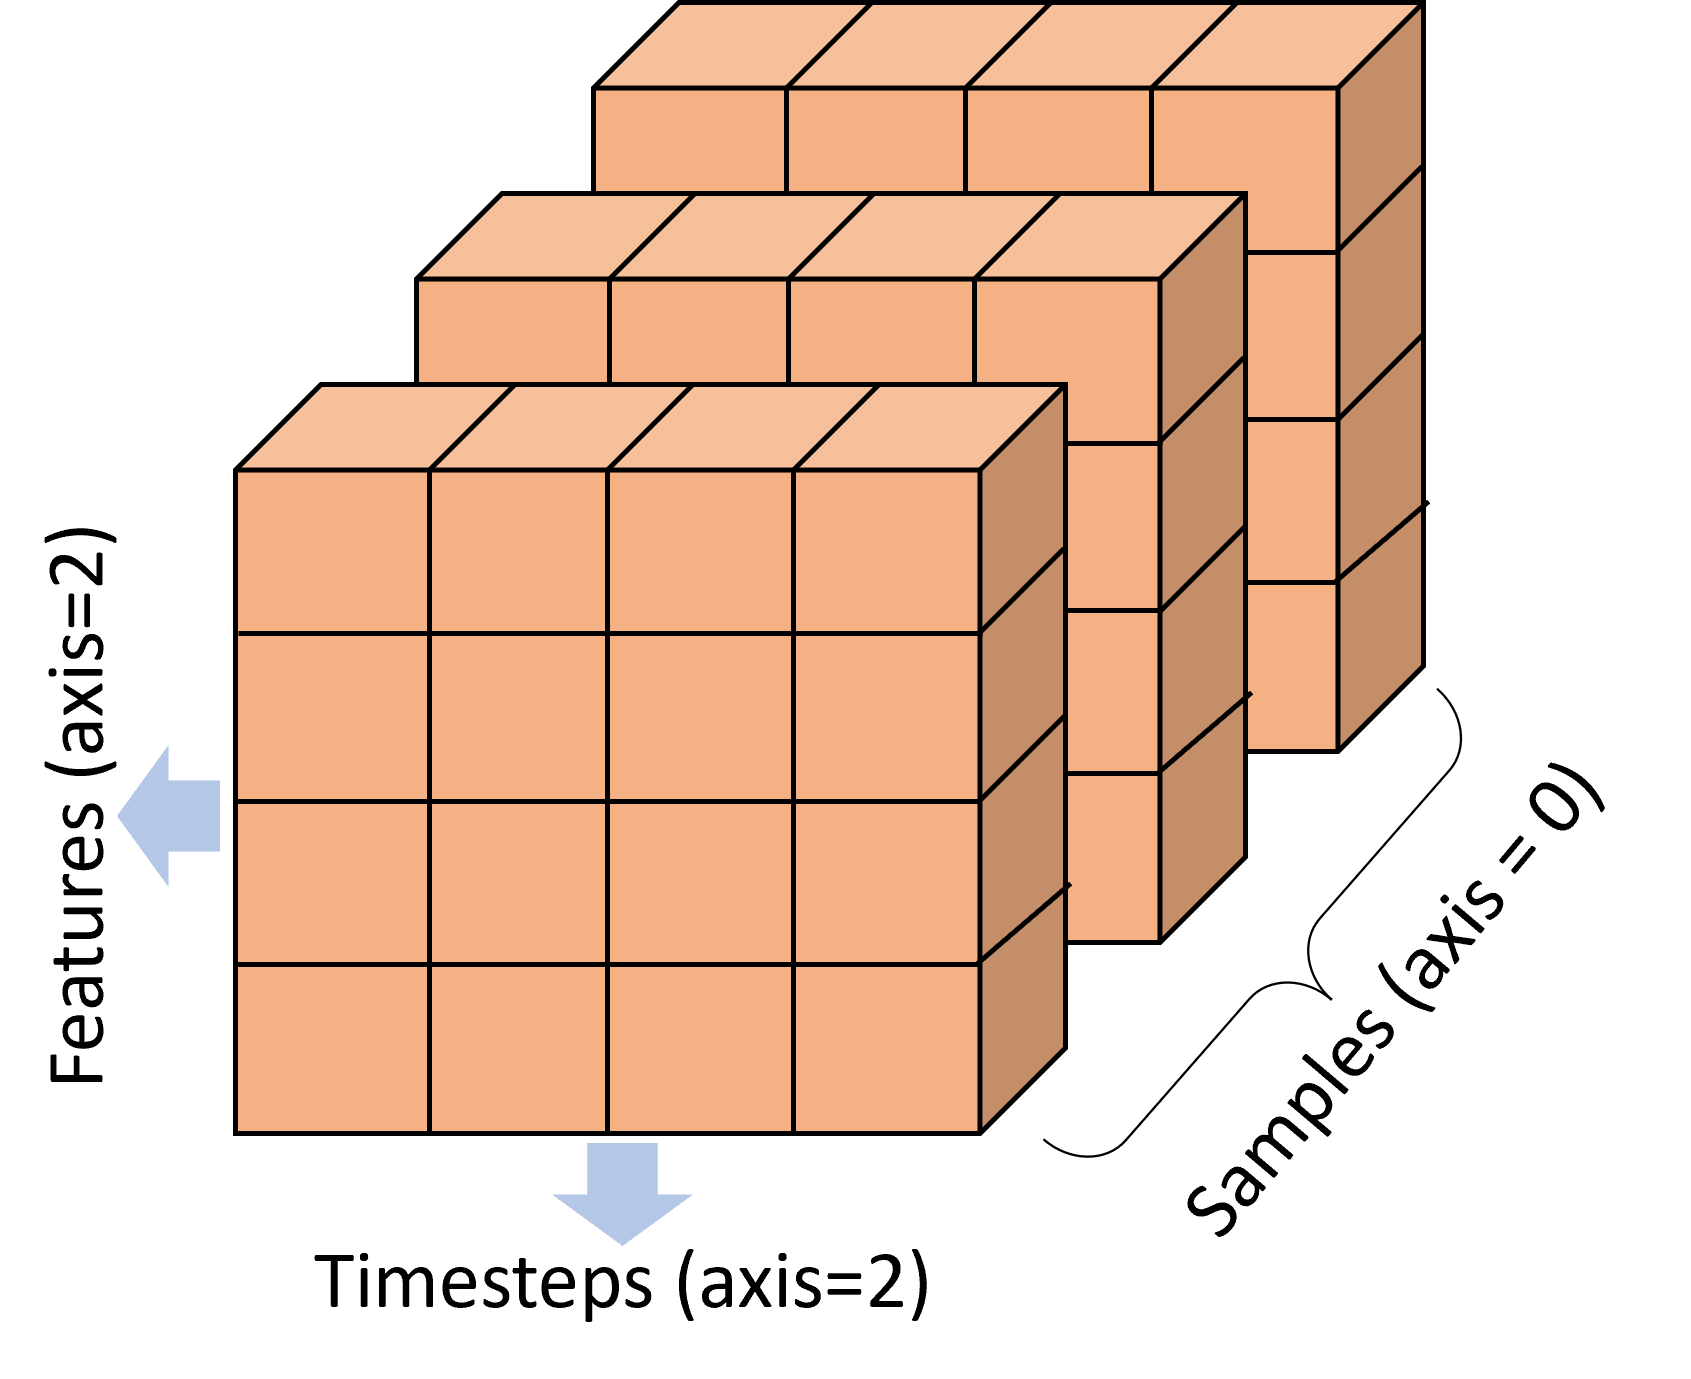
\includegraphics[width=0.5\linewidth]{images/samples-features-timesteps.png}
    \caption{Time series data represented as 3D tensors}
    \label{fig:ts_3d_data}
\end{figure}
\begin{lstlisting}[language=Python]
# Simulating streamflow data
streamflow = np.random.random((100, 1,3650))
# Extract data for the first 5 locations and the first 365 days (1 year)
subset = streamflow[:5, 0, :365]
print(subset.shape)  # Output: (5, 1, 365)
\end{lstlisting}
\end{itemize}

\begin{itemize}
    \item \subsubsection{Example 4: Satellite Image Data} 
    Satellite images are typically stored as 3D tensors (height, width, channels) or 4D tensors (batch size, height, width, channels) for a collection of images.
    In a land-cover classification example dataset of 200 satellite images, each with a resolution of 128x128 pixels and three RGB channels, would be stored as a 4D tensor of shape \texttt{(200, 128, 128, 3)}, in the format \texttt{(samples, width, height, channels)} as shown in Figure \ref{fig:4d-image-tensor}.
    \begin{lstlisting}[language=Python]
# Simulating a batch of satellite images
satellite_images = np.random.random((200, 128, 128, 3))
# Extract the first 50 images
batch_images = satellite_images[:50]
print(batch_images.shape)  # Output: (50, 128, 128, 3)
\end{lstlisting}
\end{itemize}

\begin{figure}
    \centering
    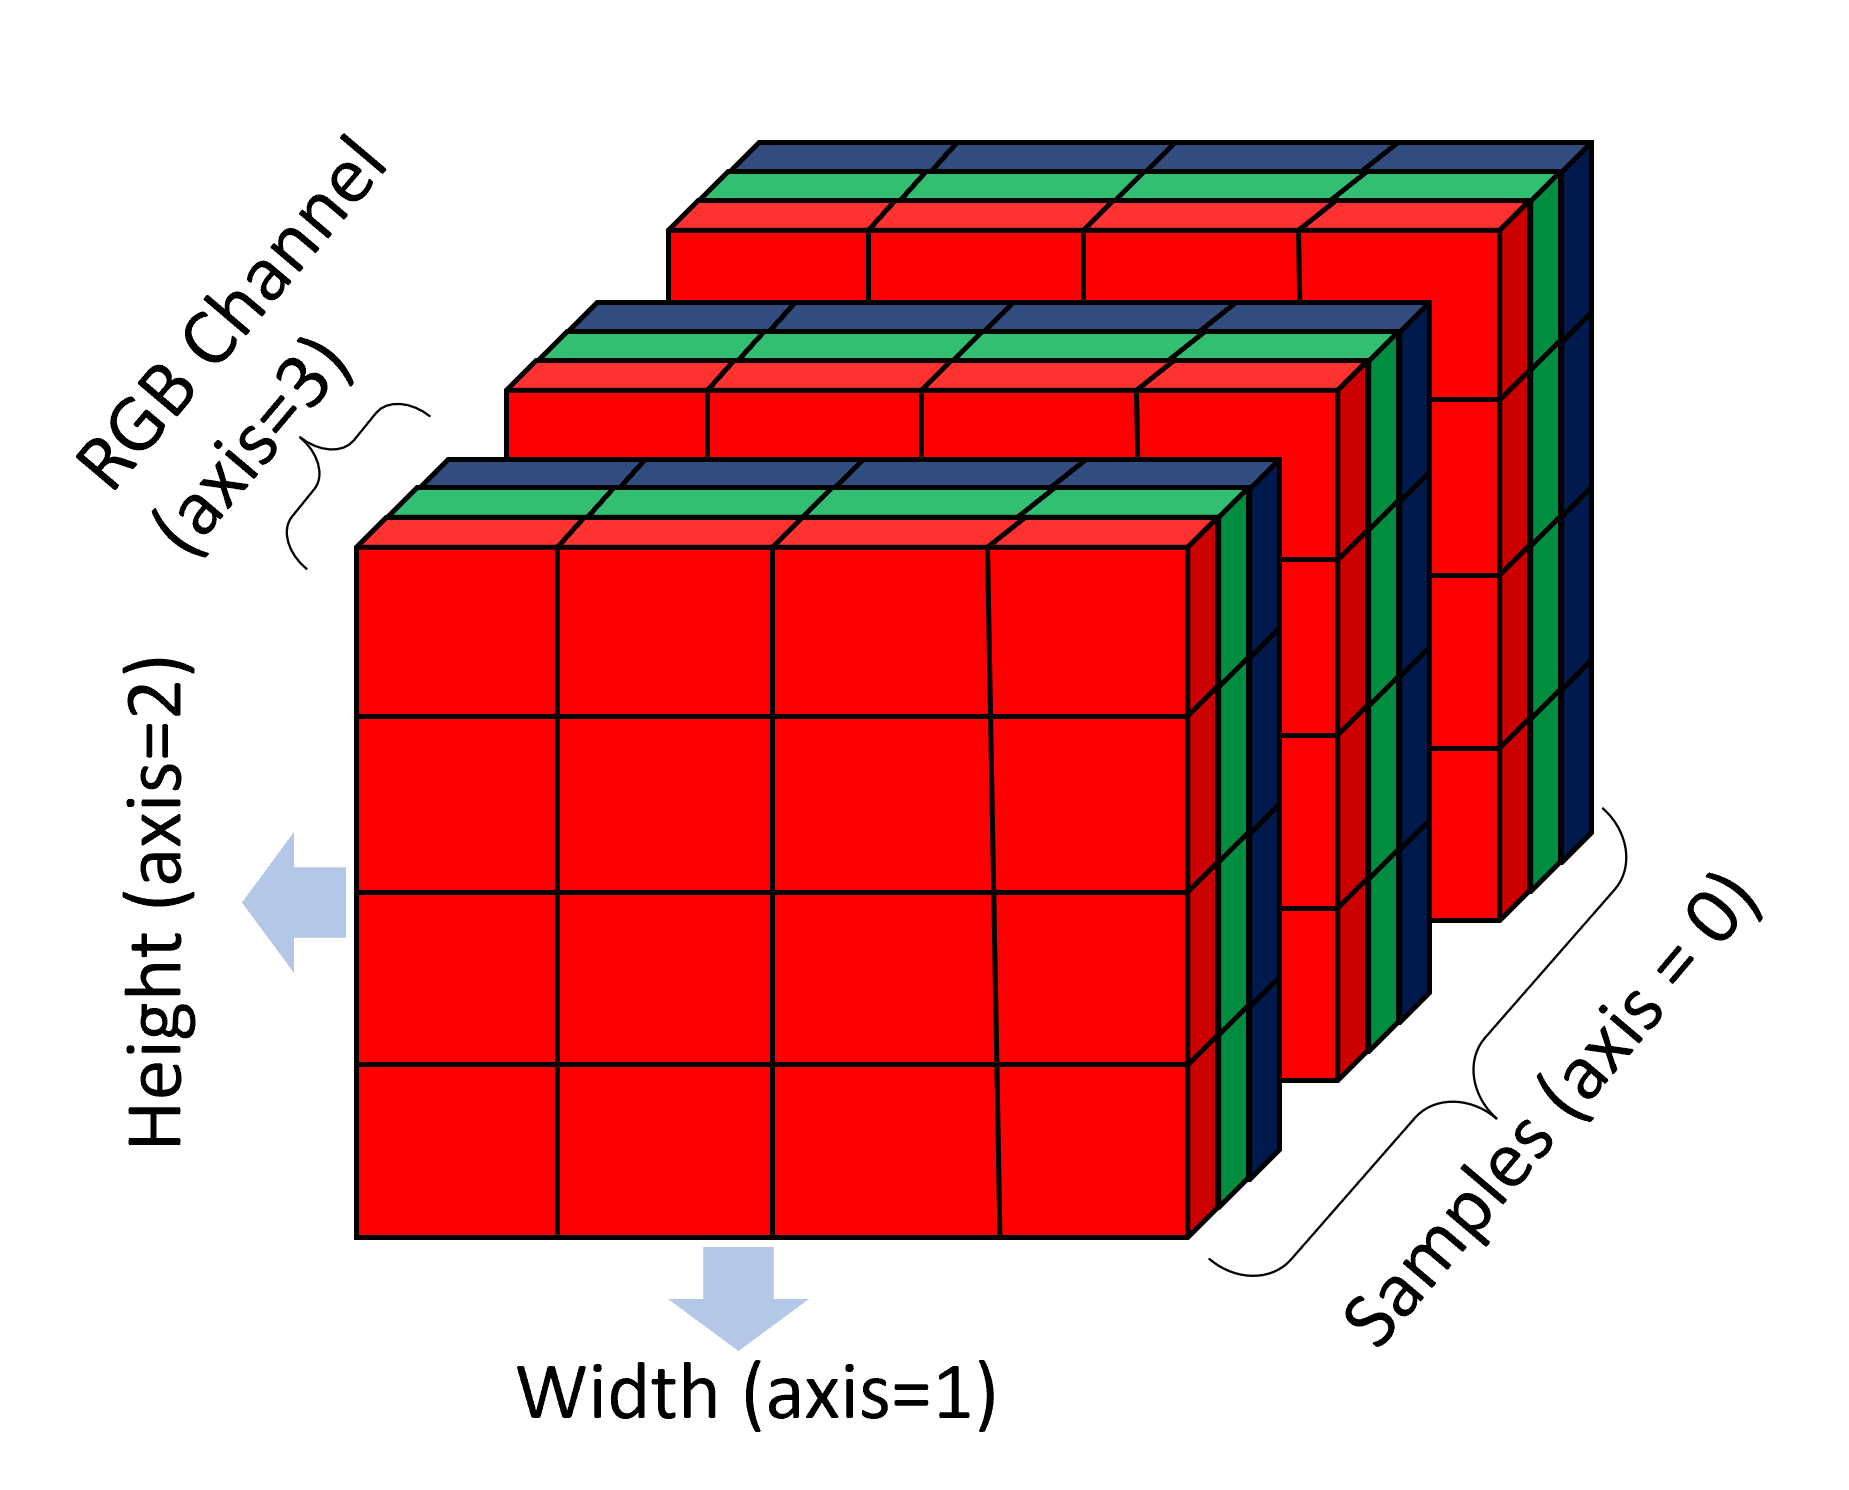
\includegraphics[width=0.5\linewidth]{images/4d-image-tensor.png}
    \caption{A 4D Image tensor data representation}
    \label{fig:4d-image-tensor}
\end{figure}





\section{Tensor Operations}


Much like computer programs are composed of simple operations on binary inputs (such as AND, OR, and XOR), deep learning models are built by applying tensor operations to numerical data. These operations are the foundation for all transformations a neural network performs. Tensor operations allow us to efficiently manipulate climate and earth science data, enabling tasks like precipitation prediction, satellite image classification, or hydrological time-series analysis.

In this section, we’ll cover the essential tensor operations—element-wise operations and broadcasting—through practical examples relevant to hydrology and remote sensing.

\subsection{Element-Wise Tensor Operations}

Element-wise operations are the simplest type of tensor operations. They involve applying a function independently to each element of a tensor or between corresponding elements of two tensors with the same shape.

\textbf{Example: Computing the Temperature Difference Between Two Grids}  
Suppose we have two temperature grids representing daily maximum and minimum temperatures (°C) over a region. These grids are stored as 2D tensors of shape \texttt{(100, 100)}, where rows and columns correspond to latitude and longitude. To compute the daily temperature range, we perform an element-wise subtraction.

\begin{lstlisting}[language=Python]
import numpy as np

# Simulated temperature grids
temp_max = np.random.random((100, 100)) * 40  # Max temperature
temp_min = np.random.random((100, 100)) * 20  # Min temperature

# Compute temperature range
temp_range = temp_max - temp_min
print(temp_range.shape)  # Output: (100, 100)
\end{lstlisting}

Each element in the \texttt{temp\_range} tensor corresponds to the temperature range at a specific grid cell.

Other common element-wise operations include addition, multiplication, and applying functions like \texttt{np.maximum()} or \texttt{np.exp()}.

---

\subsection{Broadcasting: Simplifying Operations on Tensors of Different Shapes}

In many real-world cases, tensors with different shapes need to interact. Broadcasting is a mechanism that allows smaller tensors to be automatically expanded to match the shape of larger tensors, without duplicating data in memory.

\textbf{Example: Adding a Rainfall Bias Across Multiple Regions}

Consider a dataset where daily rainfall data for 30 days is stored as a 2D tensor \texttt{rainfall} of shape \texttt{(30, 100)}, where rows represent days and columns represent regions. Suppose we want to add a constant bias correction to each region. The bias values are stored as a 1D tensor \texttt{bias} of shape \texttt{(100,)}.

\begin{lstlisting}[language=Python]
# Simulated rainfall data (mm) and bias correction
rainfall = np.random.random((30, 100)) * 50  # Daily rainfall
bias = np.random.random((100,)) * 2          # Bias for each region

# Add bias using broadcasting
corrected_rainfall = rainfall + bias
print(corrected_rainfall.shape)  # Output: (30, 100)
\end{lstlisting}

\textbf{How Broadcasting Works:}
1. The \texttt{bias} tensor of shape \texttt{(100,)} is reshaped to \texttt{(1, 100)} by adding a new axis.
2. The reshaped \texttt{bias} tensor is virtually repeated 30 times along the first axis to match the shape of \texttt{rainfall} (\texttt{(30, 100)}).
3. Element-wise addition is performed between the tensors.

\textit{Note:} Broadcasting happens at the algorithmic level and does not physically create new tensors, ensuring memory efficiency.

---

\subsubsection{A Practical Example in Remote Sensing}

Let’s consider satellite images with shape \texttt{(64, 3, 128, 128)}, representing a batch of 64 images with 3 color channels (RGB) and dimensions 128x128 pixels. We wish to normalize each pixel intensity by subtracting the mean intensity of its channel.

\begin{lstlisting}[language=Python]
# Simulated batch of images
images = np.random.random((64, 3, 128, 128)) * 255

# Mean intensity per channel
channel_mean = images.mean(axis=(0, 2, 3), keepdims=True)

# Normalize using broadcasting
normalized_images = images - channel_mean
print(normalized_images.shape)  # Output: (64, 3, 128, 128)
\end{lstlisting}

Here, the mean tensor \texttt{channel\_mean} is broadcasted to match the shape of \texttt{images}, enabling efficient subtraction across all pixels.

---

\subsection{Why Tensor Operations Matter in Hydrology}

Tensor operations are essential for:
\begin{itemize}
    \item \textbf{Analyzing Spatial Data:} Compute statistics, such as temperature ranges or precipitation anomalies, over grids.
    \item \textbf{Normalizing Datasets:} Prepare remote sensing images or time-series data for model training.
    \item \textbf{Efficient Computation:} Perform complex operations on large datasets without duplicating memory.
\end{itemize}

These operations are the building blocks for designing and training deep learning models tailored to hydrology and earth sciences.


\section{How Neural Networks Learn: Optimization Basics}



\chapter{Introduction to Machine Learning}
\begin{itemize}
    \item Key ML concepts: supervised, unsupervised, and reinforcement learning.
    \item Common algorithms: linear regression, decision trees, SVMs, etc.
    \item Preparing datasets for ML.
\end{itemize}

\chapter{Getting Started with Neural Networks}
\begin{itemize}
    \item Basic structure of neural networks.
    \item Activation functions, loss functions, and optimizers.
    \item Training, validation, and evaluation of models.
\end{itemize}

\part{Deep Learning for Time Series in Water Science}

\chapter{Introduction to RNNs and LSTM}
\begin{itemize}
    \item Basics of Recurrent Neural Networks (RNNs).
    \item Long Short-Term Memory (LSTM) networks and their advantages.
    \item Applications in hydrological modeling.
\end{itemize}

\chapter{Autoencoders}
\begin{itemize}
    \item Introduction to autoencoders and their types (vanilla, sparse, denoising).
    \item Demonstrations on hydrological data.
\end{itemize}

\chapter{Sequence-to-Sequence Prediction with LSTMs}
\begin{itemize}
    \item Encoder-decoder architectures.
    \item Bidirectional LSTMs and stacked LSTMs.
    \item Real-world applications in water resource prediction.
\end{itemize}

\chapter{Attention Mechanisms}
\begin{itemize}
    \item Introduction to attention.
    \item Applications in time-series data for hydrology.
\end{itemize}

\chapter{State-of-the-Art Transformer Models for Time Series Prediction}
\begin{itemize}
    \item Introduction to transformer models.
    \item Applications in time-series prediction and generation.
\end{itemize}

\part{Deep Learning for Image Data}

\chapter{Convolutional Neural Networks (CNNs) for Image Analysis}
\begin{itemize}
    \item Basics of CNNs.
    \item Applications to remote sensing and hydrological imagery.
\end{itemize}

\chapter{LULC Classification}
\begin{itemize}
    \item Land Use Land Cover (LULC) mapping.
    \item Demonstrations using remote sensing imagery.
\end{itemize}

\chapter{Anomaly Detection in Remote Sensing Data}
\begin{itemize}
    \item Detecting anomalies in hydrological and climate data.
    \item Examples using satellite imagery.
\end{itemize}

\chapter{Digital Elevation Model (DEM) and LiDAR Data Analysis}
\begin{itemize}
    \item Processing DEM and LiDAR datasets.
    \item Applications in flood mapping and terrain analysis.
\end{itemize}

\part{Recent Advances in Deep Learning}

\chapter{Explainable AI (XAI) for Hydrological Models}
\begin{itemize}
    \item Introduction to XAI.
    \item SHAP and Integrated Gradients for feature importance.
    \item Real-world examples: drought prediction and vegetation health.
\end{itemize}

\chapter{Physics-Guided Deep Learning (PGDL)}
\begin{itemize}
    \item Combining physics-based and data-driven models.
    \item Applications in hydrology: rainfall-runoff modeling and water level prediction.
\end{itemize}










Deep Learning For Hydrology, Water Resources, Envrionmental, Climate and Earth science domains: Theory and practice with Python


Table of Contents:
Preface:
Acknowledgments:
About the book: about Who should read this book, roadmap, software reqyirements, hardwares, and Source Code examoles. 
The book is filled with varuous real world data problems and diverse priblems like: 
(1) drought classification, (2) Rainfall runoff modeling, (3) hourly temperature prediction, (4) reservior water level classification/prediction, (5) LULC classification, (6) SM prediction, (7)  heatwave classification, (8) DEM or Lidar data, (9) vegetation health detection (10) drought prediction and monitoring in real time. 
About the authors:


The book is basically divided into 3 parts broadly. 
Part I: Fundamentals of Deep Learning

Part II: Deep Learning for Time series in Water Science
part III: Deep Learning for image types like remote sensing imagery classification of images keep a small heading for this.. 

Part IV: recent advances in Deep learning like XAI or interpretable DL, Physics guided deep learning 

Part I: 

Chapter 1: Introduction to Python (make a detailed outline here we will cover few important stuffs that will help the readers in understand the python codes throughout this book)

Chapter 2: What is Deep Learning? 

Chapter 3: Setting the stage: The mathematical Building blocks of Deep Learning

Chapter 4: Introduction to Machine Learning

Chapter 5: Getting Started from the Neural Networks

Part 2: Deep learning for Time series 

Chapter 6:Introduction to RNNs and LSTM

Chapter 7: Autoencoders and demonstrate the capability of various types of AEs.

Chapter 8: Sequence to sequyence prediction with encoder decoder LSTM, biLSTM, Stacked LSTM.

Chapter 9: Attention Mechanism

Chapter 10: State-of-the-art transformer Models for time series prediction and generation

part III: DL for image from remote sensing may be or whatever title u think is good. 

basically this part will be for the remotesensing image based data. 
here we demonstrate the LULC classification, ANomaly detection, and as different types of chapters.. of DEM mapping something we will find.. 
Use of basically CNN variants. 
part IV: understanding the blackbox DL models with XAI and PGDL

Chapter 1: XAI
disucss what is XAI and we use for example the SHAP and EG methods to find somehting from the previously discusssed problems to identify the major features. 
Chapter 2: PGDL also make its outline,, 




\chapter*{Preface}
\chapter*{Acknowledgments}
\chapter*{About the Book}

Also, most of the deep learning books available in the market are focused on delivering deep learning concepts based on natural language processing and image analysis. However, the water and earth system science domains strongly require a book that focuses on the time series problems because as earth or climate or water scientists we deal with time series data across many scenarios. Additionally, we require understanding and processing the image data to get insights from the remote sensing products for topics related to semantic segmentation, LULC classification, and anomaly detection problems. 
There are a few books that have been recently published to give the readers the essence of deep learning. Although they have explained the theories, however, these books are full of unnecessary mathematical equations and devoid of intuitions. Additionally, there are no coding examples to demonstrate that this is a great book. Mostly, they focus on a literature review and developing a very simple and rudimentary understanding of deep learning. However, we provide in-depth coding examples with real-world data in detail. There are several and a variety of examples presented. 


This book is designed for anyone passionate about applying deep learning techniques to hydrology, water resources, climate science, geology, earth sciences, remote sensing, and related domains. Whether you’re a researcher, student, or professional, this book will provide immense value by exploring how deep learning can address real-world problems in these fields.

This is a practical, hands-on guide to deep learning that avoids overly complex mathematical notation. Instead, it emphasizes intuition and understanding through clear explanations and step-by-step Python code examples. By following this book, you’ll learn to build deep learning models using the \textit{TensorFlow} and \textit{Keras} frameworks, with a focus on solving domain-specific challenges. Even if you prefer \textit{PyTorch}, the foundational knowledge and practical applications in this book will serve as a robust resource for tackling similar problems.

\section*{Real-World Problems Explored in This Book}
The book is packed with examples drawn from real-world hydrological and environmental challenges, such as:
\begin{enumerate}
    \item Drought classification.
    \item Rainfall-runoff modeling.
    \item Hourly temperature prediction.
    \item Reservoir water level prediction/classification.
    \item Land Use Land Cover (LULC) classification.
    \item Soil moisture prediction.
    \item Heatwave classification.
    \item Digital Elevation Model (DEM) and LiDAR data processing.
    \item Vegetation health detection.
    \item Drought prediction and monitoring in real time.
\end{enumerate}

\section*{Who Should Read This Book?}
This book is for:
\begin{itemize}
    \item \textbf{Hydrologists, climate scientists, geologists, and remote sensing professionals} who want to learn how to apply deep learning techniques to their data-driven problems.
    \item \textbf{Students and researchers} looking for an intuitive and accessible introduction to deep learning concepts and applications in environmental and earth sciences.
    \item \textbf{Data scientists and machine learning practitioners} who want to expand their expertise into domain-specific problems, such as water resource management and climate modeling.
    \item \textbf{Professionals transitioning to deep learning} and seeking practical examples to get started with TensorFlow and Keras.
\end{itemize}

No advanced mathematics background is required to understand this book; high school–level mathematics is sufficient. Readers should, however, have basic proficiency in Python programming and familiarity with libraries like NumPy. For those new to machine learning or deep learning, this book introduces the necessary foundations from scratch.

\section*{What You'll Learn}
After reading this book, you’ll:
\begin{itemize}
    \item Have a solid understanding of deep learning concepts and their applications in hydrology, climate science, and related domains.
    \item Be able to use TensorFlow and Keras to build, train, and evaluate deep learning models for diverse real-world problems.
    \item Understand key workflows, best practices, and challenges in applying deep learning to hydrological and environmental data.
    \item Gain practical skills in solving problems involving time series, spatial data, and remote sensing imagery.
\end{itemize}

Even if you are using PyTorch, this book will still serve as an exceptional resource to understand the concepts and workflows required for deep learning in environmental sciences. The examples provided can be adapted to your preferred framework, making this book a valuable asset regardless of your tools of choice.

\begin{mdframed}[linewidth=1pt, linecolor=gray, backgroundcolor=gray!5]
\textbf{Note:} While this book focuses on TensorFlow and Keras, the problem-solving strategies and examples are framework-agnostic. Readers using PyTorch or other deep learning libraries can still gain immense insights and apply the concepts discussed here effectively.
\end{mdframed}

This book offers not just a theoretical understanding of deep learning but also equips you with practical tools to address some of the most pressing challenges in hydrology, water resources, and environmental sciences.

\input{preface/about author}

\chapter{Introduction to Python}
\section{Why Python for DL?}
Python is our language of choice for hydrology and water resources engineering, offering a blend of simplicity and powerful functionality. Its straightforward syntax is easy for beginners to grasp, which contributes to its popularity in scientific fields, including machine learning. One of Python's greatest strengths is its extensive array of libraries. Libraries like NumPy, Pandas, and Matplotlib simplify tasks related to data handling, analysis, and visualization, making them less daunting and more efficient. These tools are crucial for hydrologists dealing with large and complex datasets.

Moreover, Python is the preferred language for TensorFlow and Keras, two of the most prominent libraries for DL. Their integration allows for advanced computational models, essential for modern hydrological research and applications. The combination of Python with these libraries opens up a world of possibilities in predictive modeling and environmental data analysis. In the following sections, we'll cover the basics of Python and these powerful libraries. For those already familiar with Python, you might choose to skim or skip these sections and proceed to the next chapter, where we dive deeper into specific hydrological applications using Python.

\section{Getting Started with Python}
\subsection{Installing Python and Setting Up the Environment}
To begin your journey with Python, the first step is installing the Python interpreter. You can download the latest version of Python from the official website: python.org. The website provides installation packages for various operating systems, including Windows, macOS, and Linux. Follow the installation instructions specific to your operating system. During installation, ensure that you select the option to add Python to your system's PATH, which makes it accessible from the command line.

For a more visual and guided setup process, consider watching tutorial videos on YouTube. Many content creators provide step-by-step guides on installing Python and setting up the environment, catering to different operating systems. These videos can be particularly helpful if you're new to installing software or configuring development environments. Opting for a video tutorial is often the quickest way to ensure a smooth and correct setup, allowing you to start coding in Python without unnecessary delays.

\subsection{Python IDEs and Editors}
While Python code can be written in any text editor, using an Integrated Development Environment (IDE) can significantly enhance your coding experience. IDEs provide features like syntax highlighting, code completion, and debugging tools. Some popular Python IDEs include PyCharm and Visual Studio Code. However, for DL applications, especially in hydrology and water resources engineering, we recommend using Jupyter Notebooks.

\subsection{Jupyter Notebooks: The Preferred Environment for DL}
We recommend using Jupyter Notebooks for several reasons, especially for beginners and those working on DL projects:

Interactive Development: Jupyter Notebooks provide an interactive development environment, allowing you to write and execute code in chunks (cells).
Experimentation and Visualization: They are ideal for experimentation, data analysis, and visualization—all crucial in DL.
Documentation and Sharing: Notebooks facilitate documentation and sharing of code, results, and explanations, making them excellent for educational purposes and collaborative projects.
For a cloud-based solution, Google Colab stands out as an exceptional choice. It offers a comparable interactive experience without the need for installation and is accessible from any web browser. Notably, Colab facilitates free GPU access, a boon for executing complex DL models. Discover more about \href{https://colab.research.google.com}{Google Colab}.

Both platforms, Jupyter Notebooks and Google Colab, support easy sharing and collaboration, including direct integration with GitHub. This feature is invaluable for DL practitioners, educators, and students alike, democratizing access to advanced computational resources and fostering a collaborative learning environment. As you delve into this book, utilizing Jupyter Notebooks will enrich your understanding of DL's practical applications in hydrology and water resources engineering, enhancing both learning and discovery.

\subsection{Writing Your First Python Program}
Once your Jupyter Notebook environment is set up, it's time to write your first Python program. Open Jupyter Notebook in your browser, create a new notebook, and you're ready to start coding. You can begin with a simple program, like printing a message:

\begin{lstlisting}[language=Python]
print("Welcome to DL in Hydrology")
output: [1] Welcome to DL in Hydrology
\end{lstlisting}

Type this into a Jupyter cell and execute it by pressing 'Shift + Enter'. Congratulations, you've just run your first Python program!

\section{Recommended Hardwares and GPU}

DL tasks in hydrology, such as predicting rainfall patterns, modeling watershed dynamics, or simulating flood events, require significant computational power. This section provides guidelines on the necessary hardware to efficiently run DL models, tailored for different levels of project complexity—from classroom projects to high-performance research applications.

\subsection{Basic Hardware for Classroom and Small Projects}
For individuals or students just starting with DL applications in hydrology:

\begin{itemize}
    \item \textbf{Processor (CPU)}: A modern multi-core processor (e.g., Intel i5 or i7, or AMD Ryzen 5 or 7) will be sufficient for basic data processing and smaller models.
    \item \textbf{Memory (RAM)}: At least 8GB of RAM, though 16GB is recommended for better multitasking and handling larger datasets.
    \item \textbf{Storage}: SSD storage of at least 256GB for faster data access and program loading times.
\end{itemize}

\subsection{Advanced Hardware for Research and Large Projects}
For researchers and larger projects that require more intensive computations and data handling:

\begin{itemize}
    \item \textbf{Graphics Processing Unit (GPU)}: A dedicated NVIDIA GPU is crucial for accelerating DL tasks. We recommend using at least an NVIDIA RTX 3060 for moderate projects. This GPU offers excellent performance for most DL tasks without breaking the budget.
    \item \textbf{High-Performance Computing (HPC) Configurations}:
    \begin{itemize}
        \item For advanced research requiring extensive simulations and model training, consider HPC resources equipped with NVIDIA Tesla or Quadro series GPUs.
        \item Multiple GPU setups can significantly reduce model training time. Systems such as NVIDIA DGX Stations or custom builds with multiple RTX 3090s are recommended for high-end computational needs.
    \end{itemize}
\end{itemize}

\subsection{Recommendations for High-Performance Computing}
For those with access to or considering investment in high-performance computing environments:

\begin{itemize}
    \item \textbf{Cluster Configuration}: A cluster with multiple NVIDIA A100 GPUs interconnected with high-speed networking (e.g., InfiniBand) ensures that large-scale models can be trained efficiently.
    \item \textbf{Memory and Storage}: High RAM capacity (256GB or more) and fast I/O storage solutions (NVMe SSDs in RAID configuration) are crucial for handling vast datasets and simultaneous processes.
\end{itemize}

\subsection{Additional Resources}
To further explore the specifications and capabilities of recommended GPUs and to stay updated with the latest advancements in computing hardware, please refer to the following resources:

\begin{itemize}
    \item \href{https://www.nvidia.com/en-us/deep-learning-ai/products/}{NVIDIA DL GPUs}
    \item \href{https://www.intel.com/content/www/us/en/high-performance-computing/hpc-overview.html}{Intel AI and HPC Solutions}
    \item \href{https://www.amd.com/en/processors/ryzen-for-business}{AMD Ryzen Processors}
\end{itemize}

By equipping yourself with the right hardware, you can ensure that your DL models operate efficiently, allowing you to focus more on innovation and less on computational limitations.

\section{Data Structures in Python}

\subsection{Lists and Tuples}
Python provides several compound data types, useful for grouping together other values. The most versatile of these are lists and tuples, which can be written as a list of comma-separated values between square brackets for lists, or parentheses for tuples.

\subsubsection{Creating Lists and Tuples}
\begin{lstlisting}[language=Python]
# Creating a list
rainfall = [20.5, 30.2, 25.4, 12.2]

# Creating a tuple
months = ('January', 'February', 'March', 'April')
\end{lstlisting}

\subsubsection{Accessing Elements, Slicing, and List Comprehensions}
\begin{lstlisting}[language=Python]
# Accessing elements
print(rainfall[1])  # Output: 30.2

# Slicing
print(months[0:2])  # Output: ('January', 'February')

# List comprehension
squared = [x**2 for x in range(5)]
print(squared)  # Output: [0, 1, 4, 9, 16]
\end{lstlisting}

\subsection{Dictionaries}
Dictionaries are another fundamental data structure in Python. They store mappings of unique keys to values and are incredibly efficient for retrieving data.

\subsubsection{Creating and Manipulating Dictionaries}
\begin{lstlisting}[language=Python]
# Creating a dictionary
river_flow = {'Amazon': 209000, 'Nile': 2830, 'Yangtze': 31900}

# Adding a new key-value pair
river_flow['Mississippi'] = 16200
\end{lstlisting}

\subsubsection{Importance of Dictionaries in Data Handling}
Dictionaries allow for rapid data retrieval via keys and are essential for data processing tasks where relationships between elements must be efficiently established and accessed.

\subsection{Sets and Frozensets}
Sets are collections of distinct (unique) items that are useful when you want to ensure no duplicates are present.

\subsubsection{Characteristics of Sets and Their Utility}
\begin{lstlisting}[language=Python]
# Creating a set
unique_rivers = set(['Amazon', 'Nile', 'Yangtze', 'Nile'])
print(unique_rivers)  # Output: {'Yangtze', 'Amazon', 'Nile'}

# Creating a frozenset
immutable_rivers = frozenset(['Amazon', 'Nile'])
\end{lstlisting}

Sets are particularly useful in data processing for operations like union, intersection, and difference, which can help in filtering and comparing datasets.

\section{Data Structures in Python}

Data structures are fundamental ways of organizing data to ensure efficient access and modification. Python simplifies learning these fundamentals compared to other programming languages, making it an ideal choice for hydrologists and environmental scientists.

\subsection{Lists}
Python lists are versatile and can be compared to arrays in other programming languages but with the added benefit of being able to store different types of data. Lists in Python are dynamic, meaning they can grow or shrink, and they are implemented similarly to vectors in C++ or ArrayLists in Java.

\subsubsection{Basic List Operations}
\begin{lstlisting}[language=Python]
# Creating a List with hydrological data points
rainfall_mm = [20, 30, 45, 50]
print("Monthly Rainfall in mm: ")
print(rainfall_mm)

# Creating a Multi-Dimensional List for different regions
region_rainfall = [['North', 20], ['South', 30]]
print("\nRegion-Wise Rainfall:")
print(region_rainfall) 

# Accessing elements using positive and negative indexing
print("\nAccessing the first and last element:")
print(rainfall_mm[0], rainfall_mm[-1])
\end{lstlisting}

\subsubsection{List Comprehension}
List comprehensions provide a concise way to create lists. Common applications include creating new lists where each element is the result of some operations applied to each member of another sequence or iterable.

\begin{lstlisting}[language=Python]
# Using list comprehension to square numbers
squared_numbers = [x**2 for x in range(6)]
print("\nSquared numbers from 0 to 5:")
print(squared_numbers)
\end{lstlisting}

\subsection{Dictionaries}
Dictionaries in Python are hash tables that store data in a key-value pair. They provide very fast O(1) time complexity for looking up data and are particularly useful in scenarios where the dataset is large and search speed is critical.

\subsubsection{Using Dictionaries in Hydrology}
\begin{lstlisting}[language=Python]
# Creating a dictionary to store river discharge rates
discharge = {'Amazon': 209000, 'Nile': 2830, 'Yangtze': 31900}
print("River discharge rates (cubic meters per second):")
print(discharge)

# Accessing data by river name
print("\nDischarge of the Nile:")
print(discharge['Nile'])

# Using get() to safely access elements
print("\nDischarge of the Ganges:")
print(discharge.get('Ganges', 'No data available'))
\end{lstlisting}

\subsubsection{Dictionary Comprehension}
Dictionary comprehensions offer a method to succinctly create dictionaries from a set of values.

\begin{lstlisting}[language=Python]
# Creating a dictionary to map river names to their lengths
river_length = {river: length for river, length in [('Amazon', 6400), ('Nile', 6650)]}
print("\nRiver lengths in kilometers:")
print(river_length)
\end{lstlisting}

\subsection{Tuples}
Tuples are immutable sequences in Python, used to store collections of heterogeneous data. Tuples are particularly useful when you need a fixed set of elements that should not change throughout the program.

\subsubsection{Creating and Using Tuples}
\begin{lstlisting}[language=Python]
# Defining a tuple for geographic coordinates
coordinates = (40.7128, -74.0060)
print("Coordinates of New York City:")
print(coordinates)

# Single element tuple, notice the comma
single_tuple = ('single',)
\end{lstlisting}

Tuples are not just immutable lists; they can be used as keys in dictionaries or as elements in sets, which is not possible with lists due to their mutability. This characteristic makes tuples incredibly useful in high-performance computing scenarios where data integrity and speed are paramount.

These sections provide a robust introduction to Python data structures with practical examples that demonstrate their application in environmental science and hydrology. This approach not only helps in understanding Python's capabilities but also illustrates its practical benefits in scientific computing.



\chapter{Basic Concepts of Deep Learning}

In recent years, artificial intelligence (AI) and deep learning (DL) have transformed the way we approach some of the most complex challenges in hydrology, geoscience, and environmental science. These technologies have moved beyond simple predictions to achieve groundbreaking feats, such as NASA’s DL-based models for real-time global precipitation estimates and large-scale climate simulations that capture fine-grained details of weather extremes. Researchers have even developed AI-driven systems akin to generative pre-trained transformer (GPT), trained on decades of environmental data, to assist in forecasting water resource availability and identifying critical climate trends.

The promise of AI and DL in water sciences is immense. From reimagining flood preparedness with hyper-accurate early warning systems to unraveling the mysteries of groundwater depletion with global-scale models, the potential applications are as vast as they are impactful. At the same time, this field is highly competitive, with scientists racing to harness these tools to address urgent environmental issues, inform policy decisions, and secure a sustainable future.

This chapter introduces the foundational ideas of AI and DL, exploring how these tools have already reshaped water and climate sciences and the transformative possibilities that lie ahead.

\begin{figure}[!h]
    \centering
    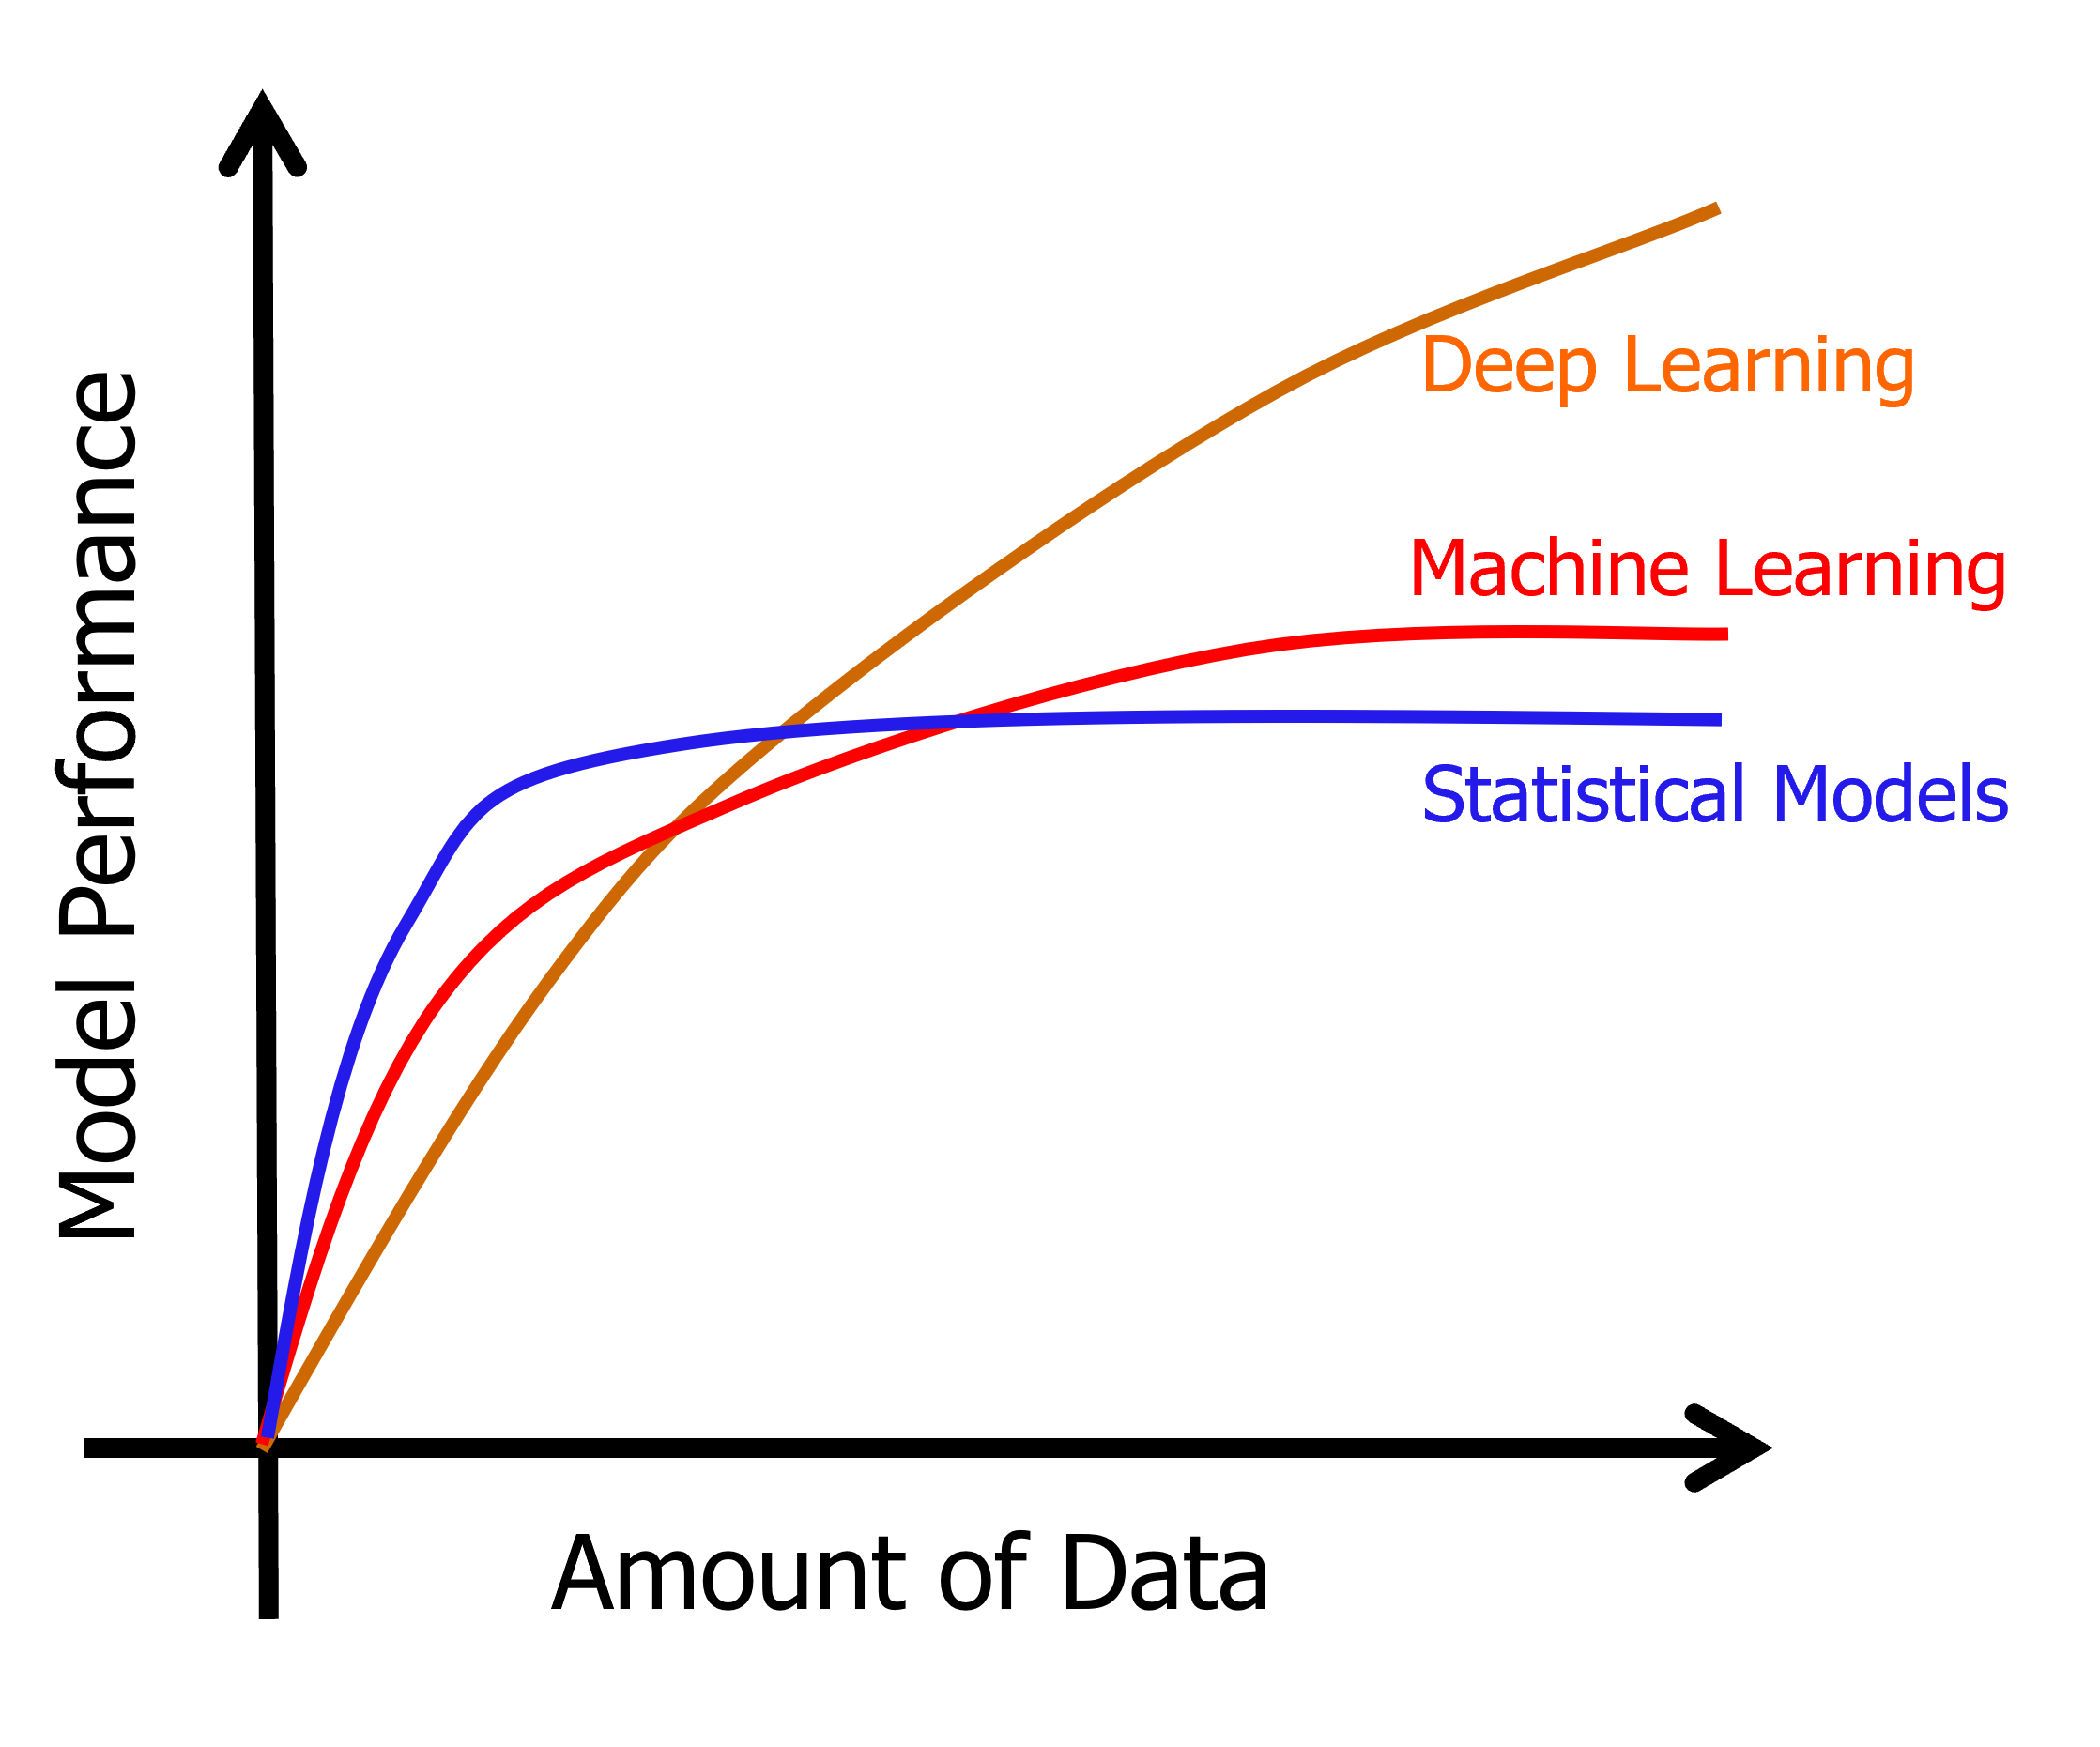
\includegraphics[width=1\linewidth]{images/What is DL.png}
    \caption{Comparison of model performance across increasing data availability for statistical models, machine learning, and deep learning}
    \label{fig:what_is_dl}
\end{figure}


\section{Understanding AI, ML, and DL: How They Relate to Each Other}
Before diving into deep learning and its applications, it’s essential to understand its roots and how it fits into the broader picture of AI and ML. Think of AI, ML, and DL as nested boxes, where each is a subset of the previous one.
\begin{figure}
    \centering
    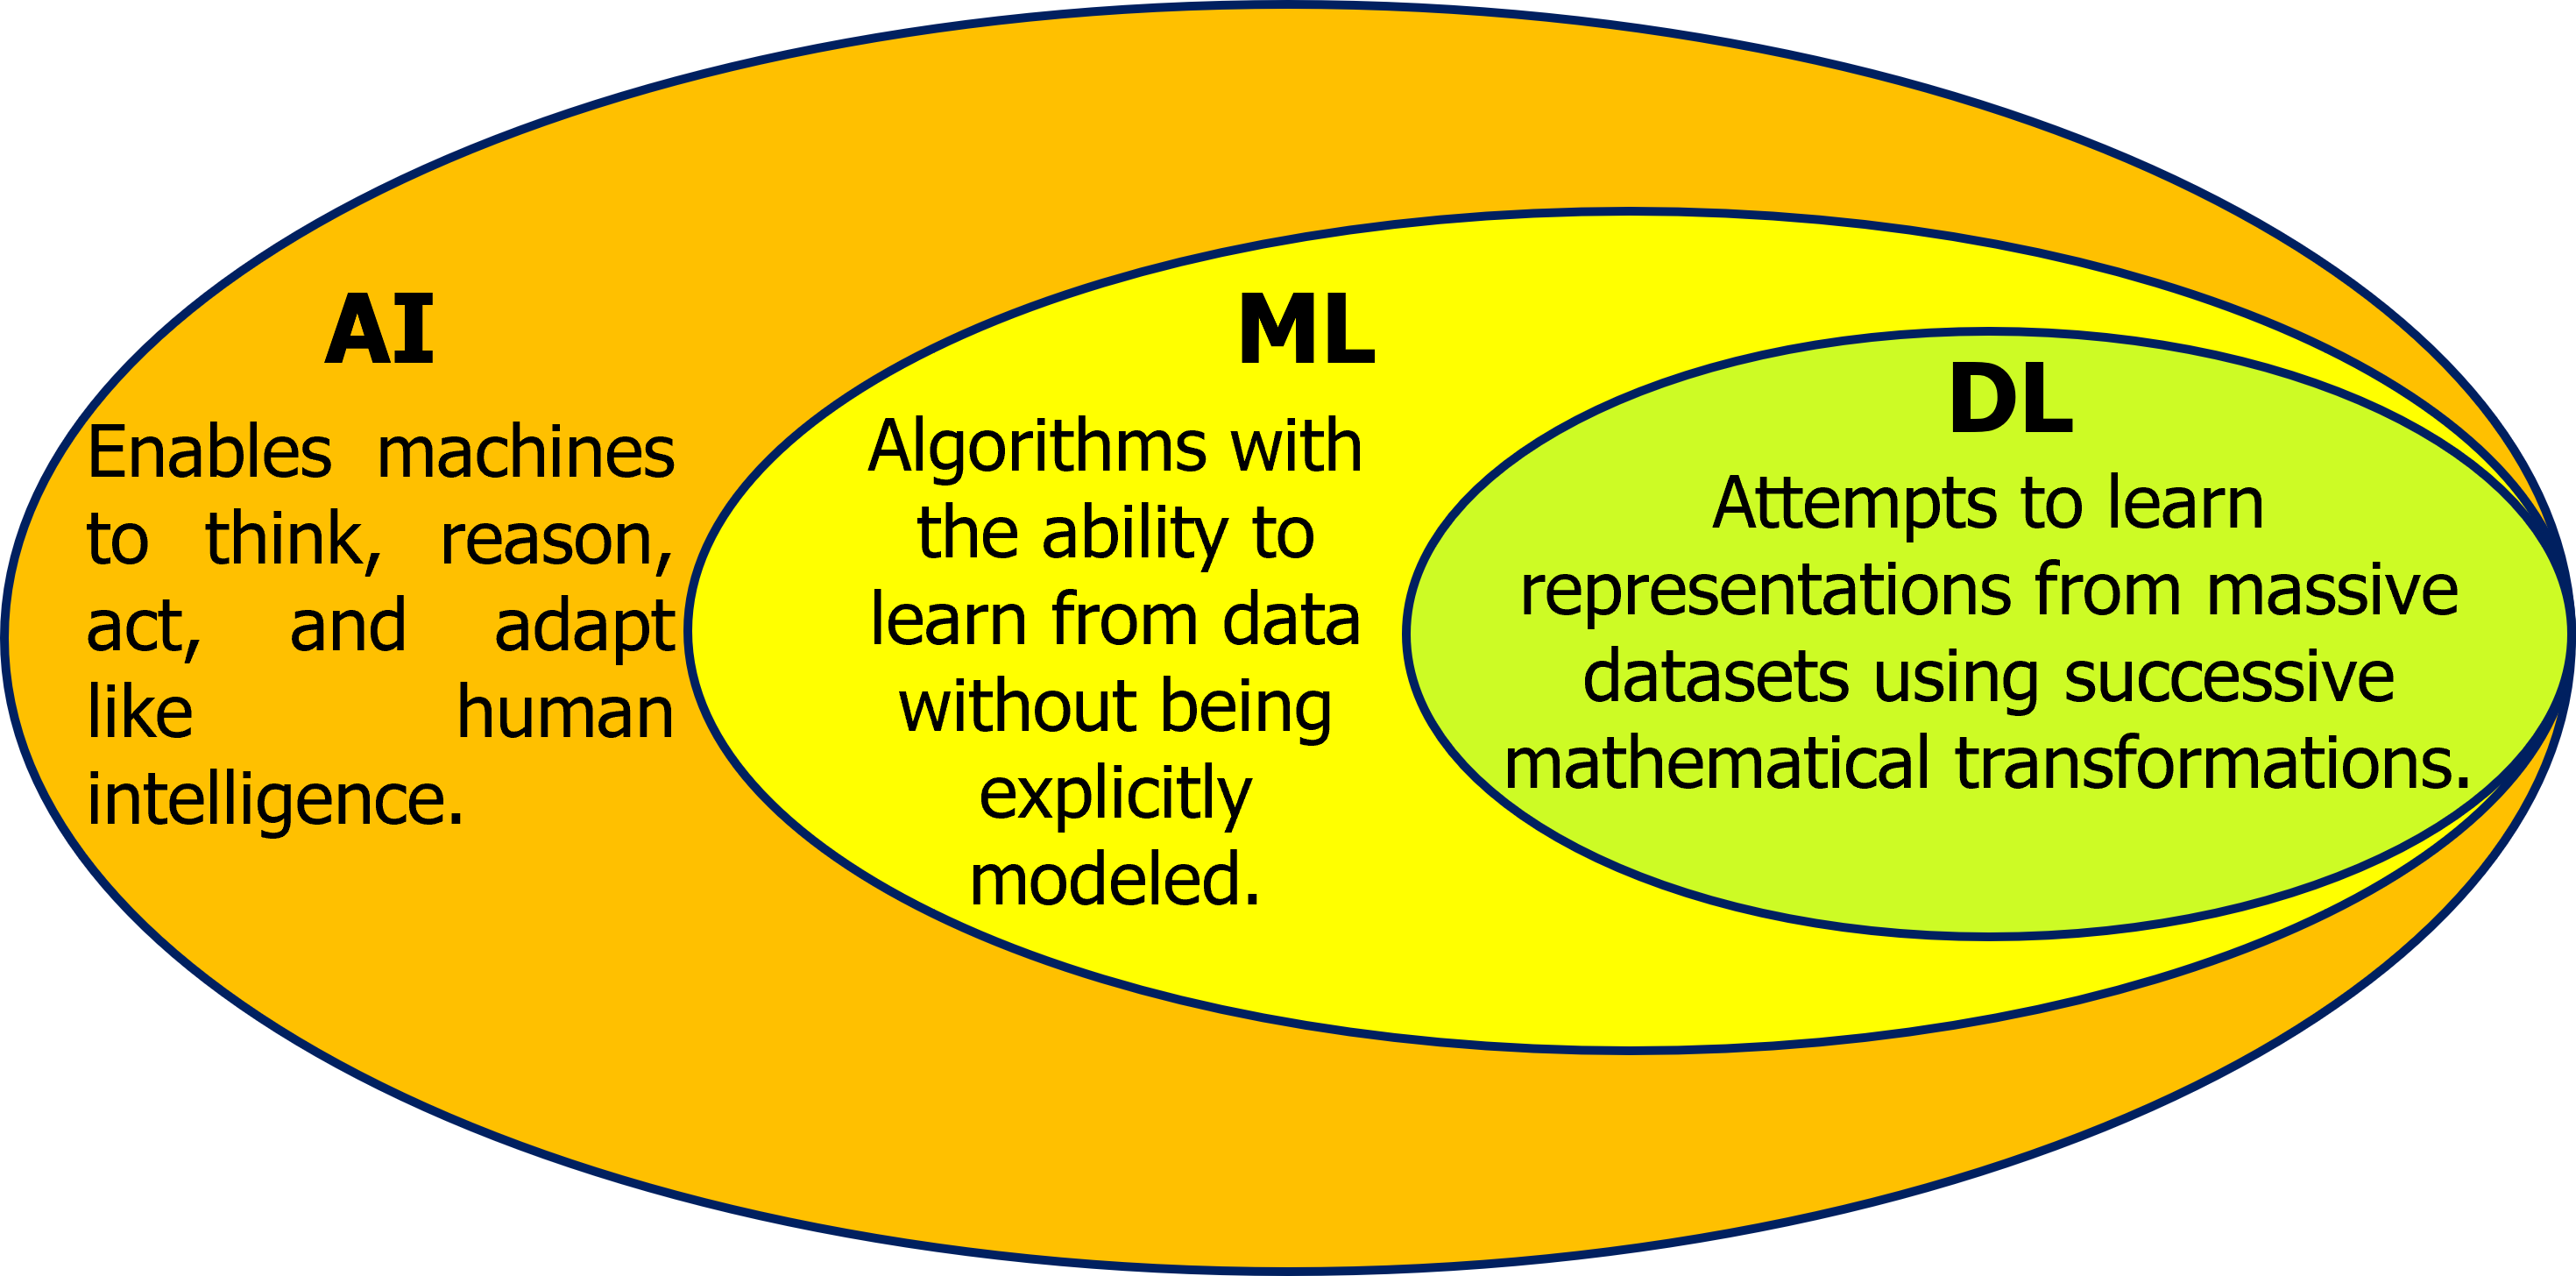
\includegraphics[width=0.99\linewidth]{images/ai-ml-dl.png}
    \caption{Illustrates the hierarchical relationship between Artificial Intelligence (AI), Machine Learning (ML), and Deep Learning (DL), with AI representing a broader field, ML as its subset, and DL as a subset of machine learning}
    \label{fig:ai-ml-dl}
\end{figure}
\subsection{Artificial Intelligence: The Big Picture}
The term Artificial Intelligence (AI) was coined in the mid-20th century, during a time when computers had only begun to show potential as tools capable of performing tasks resembling human intellect. AI broadly refers to systems designed to automate intellectual tasks typically performed by humans, such as reasoning, learning, and problem-solving.

In its earliest days, AI systems were built using hardcoded rules—a paradigm known as \textit{symbolic AI}. These systems were excellent at solving narrowly defined, logical problems, like playing chess or diagnosing straightforward faults in machinery. For example, early AI systems could be programmed to predict river discharge based on a fixed set of rules derived from historical data patterns. Another example could be simulating the operation of a water distribution network to optimize supply during drought conditions. These rule-based systems worked well for straightforward scenarios but struggled when faced with the complexity and variability of real-world problems, such as predicting extreme floods caused by unexpected climatic events.

The shortcomings of symbolic AI led to the realization that complex, fuzzy tasks—like understanding the nuances of water quality dynamics in a lake or recognizing patterns in satellite imagery of drought-stricken areas—could not be solved by explicitly defining every rule. This gave rise to new approaches like \textit{Machine Learning}, which relies on the computer learning from data rather than being explicitly programmed.

\subsection{Machine Learning(ML)}

ML emerged as a transformative step in AI's evolution. It addressed a key limitation of early AI systems, which relied on programmers explicitly defining rules for every possible situation. ML posed a new question: \textit{Could a machine learn the rules itself from data?}

This paradigm shift gave birth to a new programming approach. Instead of explicitly instructing machines, ML systems learn by example. Humans supply \textbf{input data} and the corresponding \textbf{desired outputs}, and the machine learns to infer the rules that map the inputs to the outputs. These learned rules can then be generalized to make predictions on new, unseen data. Classical programming operates as follows (see Figure \ref{fig:ml}):
\begin{enumerate}
    \item \textbf{Humans define rules} to process data.
    \item Machines apply these rules to produce outputs.
\end{enumerate}

Machine learning, on the contrary, inverts this process:
\begin{enumerate}
    \item Humans provide \textbf{ data samples and their outputs}.
    \item The machine generates the rules that connect the data to its output.
\end{enumerate}
\begin{figure}
    
    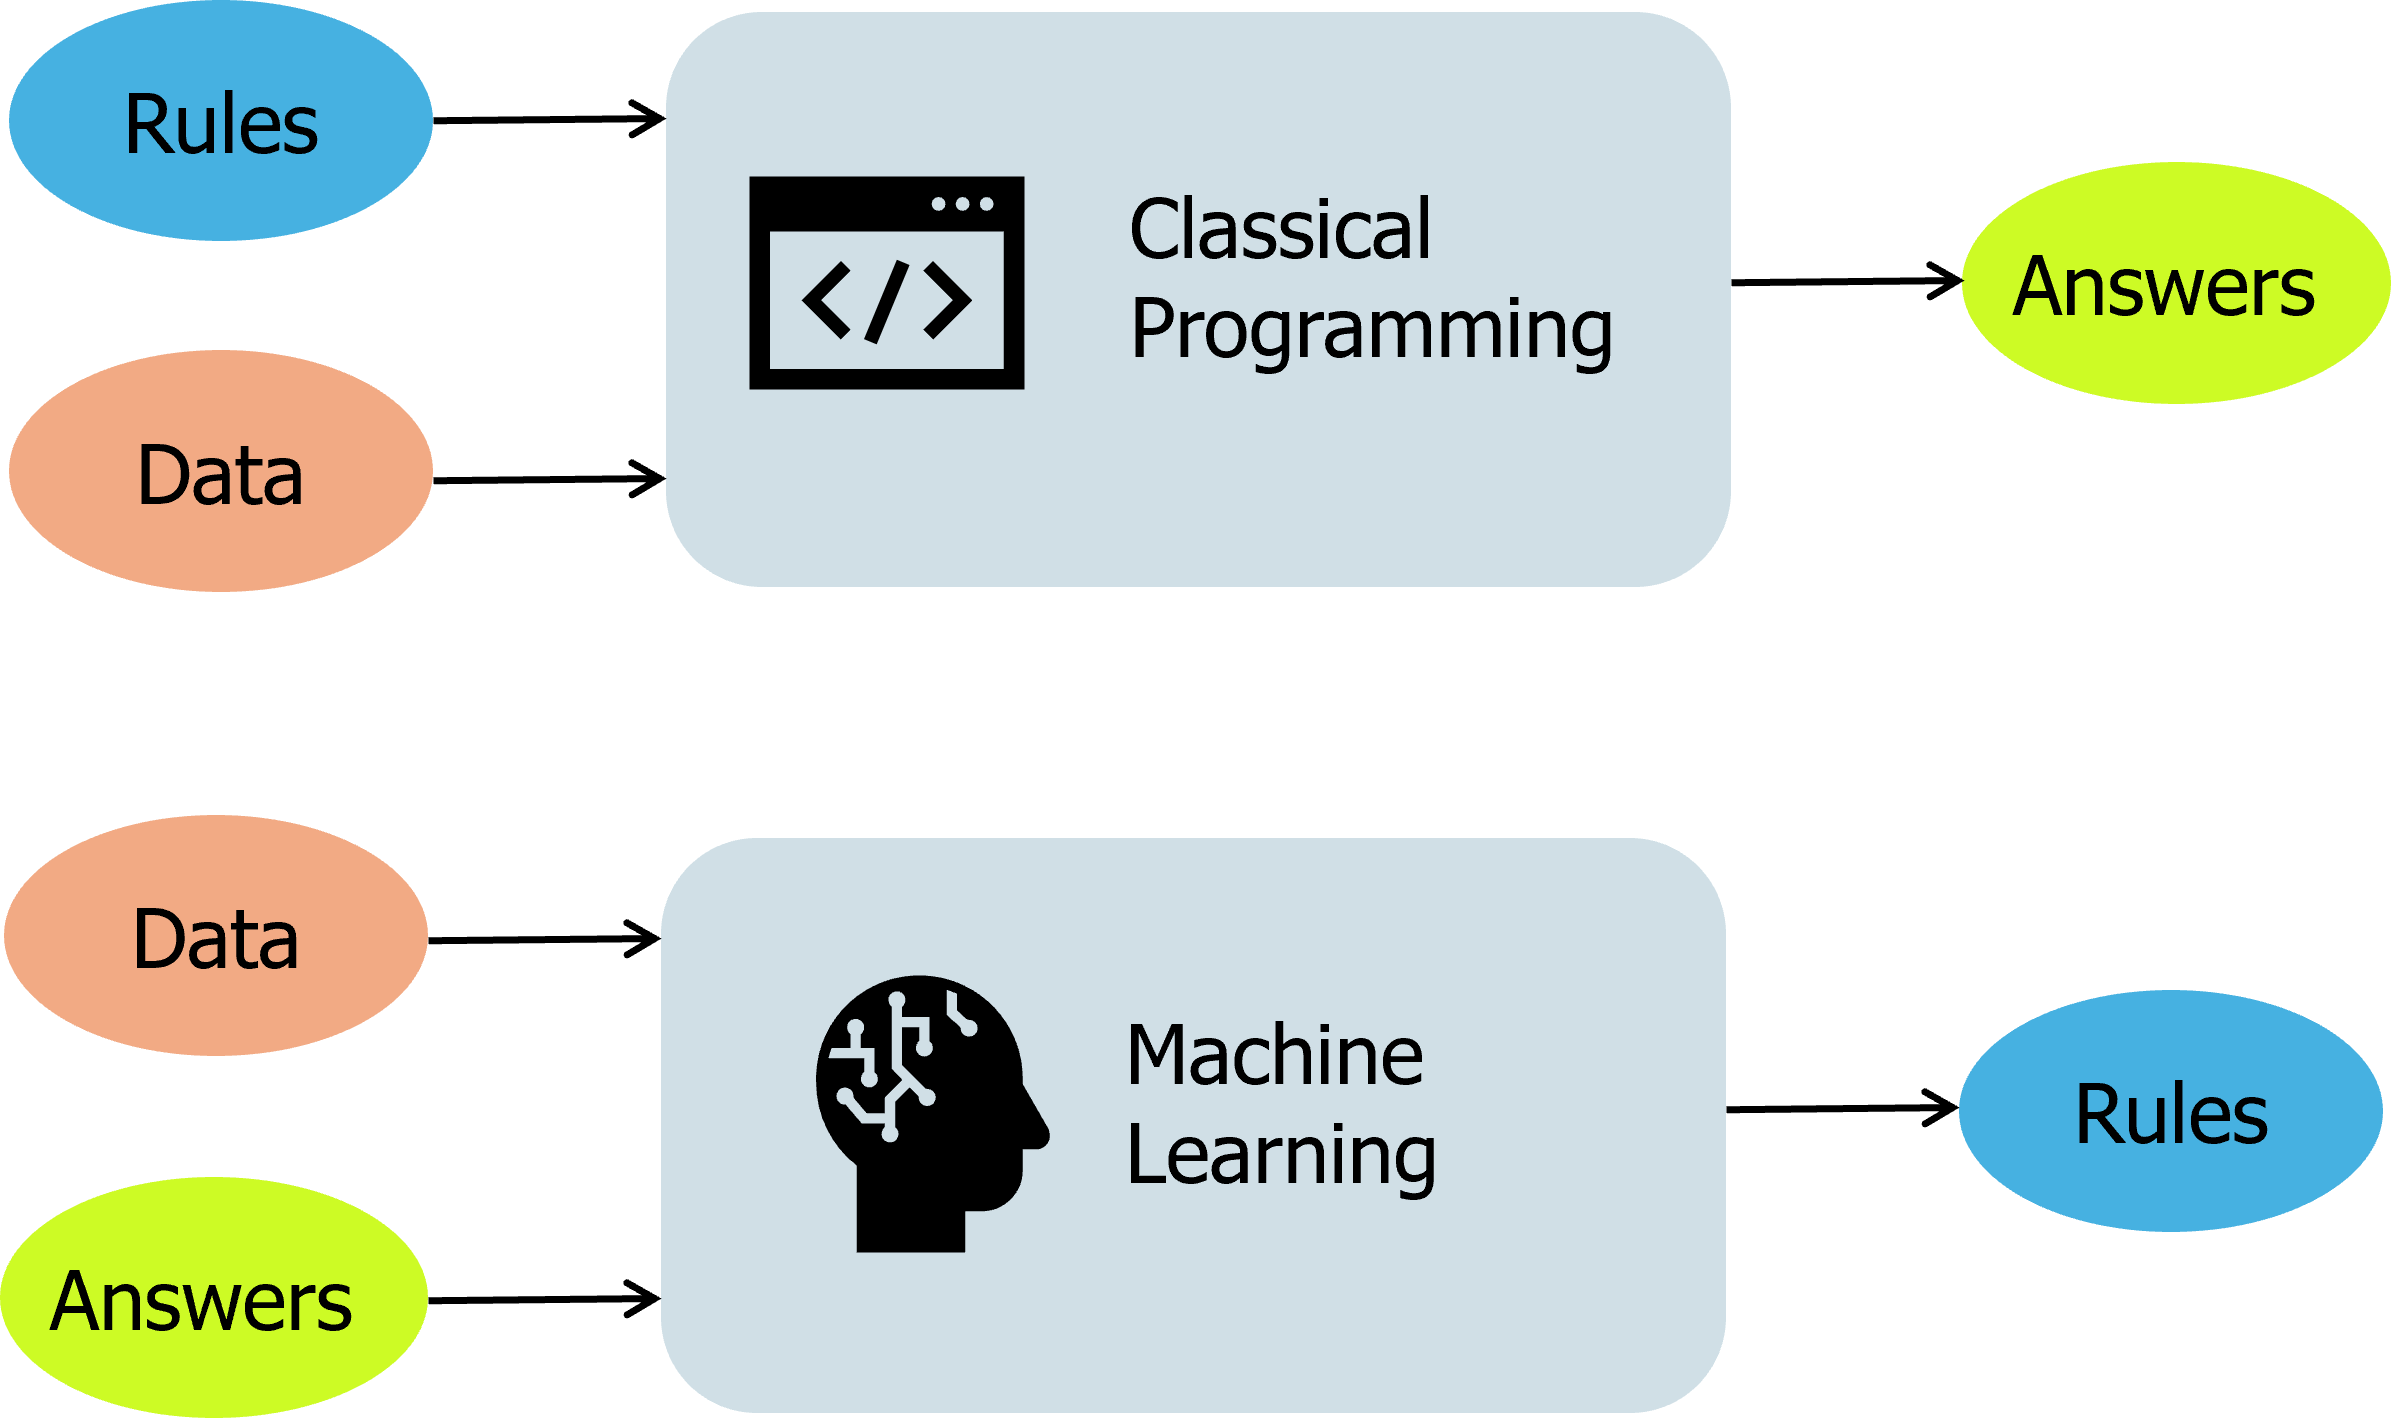
\includegraphics[width=0.75
    \linewidth]{images/ml.png}
    \caption{Classical programming vs Machine Learning (ML)}
    \label{fig:ml}
\end{figure}
This shift is similar to teaching a student by showing examples rather than lecturing about every concept. The result is a machine that can adapt and improve its performance without human intervention in the crafting of detailed instructions.

\subsubsection{Example from Hydrology}

To automate \textit{streamflow prediction}, classical programming might involve encoding complex hydrological models with explicit equations for runoff and infiltration. However, this approach struggles with unmodeled phenomena such as sudden changes in land use or climate variability.

With ML, the system is fed:
\begin{itemize}
    \item Historical data \textbf{ of rainfall and runoff} (input).
    \item Corresponding observed \textbf{streamflow values} (output).
\end{itemize}

The machine learns patterns and relationships within these data, creating a model capable of predicting stream flow under new rainfall scenarios without being explicitly programmed for every possible condition.

\subsection{Why ML Became So Popular in hydrology?}
Machine learning began to flourish in the 1990s, especially in the computer vision domain. However, its adoption in hydrology gained significant traction around 2005 and surged post-2010 due to the following factors:
\begin{itemize}
    \item \textbf{Proliferation of Diverse and Large Datasets:} Hydrology has seen an exponential increase in data availability, thanks to advancements in remote sensing technologies such as MODIS and GRACE, ground-based sensors, and climate model simulations. These multi-source, multi-scale datasets encompass high-resolution spatial and temporal data, enabling the study of nonlinear interactions across hydrological processes. ML capitalizes on such rich datasets to extract patterns and insights that traditional methods often fail to capture.
    \item \textbf{Breakthroughs in Computational Power:} The advent of high-performance computing resources, particularly GPUs (e.g., NVIDIA’s CUDA-enabled GPUs), has transformed the computational landscape. These technologies allow for efficient training of ML models on vast hydrological datasets, enabling simulations and analyses such as flood modeling, soil moisture estimation, and runoff prediction at resolutions that were once computationally prohibitive.

    \item \textbf{Capability to Handle Complexity:} Hydrological systems are inherently complex and governed by nonlinear interactions across multiple scales. Traditional statistical methods often struggle to model such complexity effectively. Machine learning, with its ability to process high-dimensional data and uncover hidden relationships, provides robust tools for prediction and inference in hydrological contexts, including flood forecasting, drought prediction, and water quality assessment.
    
    \item \textbf{Advances in Open-Source Tools and Libraries:} The widespread availability of open-source machine learning libraries like TensorFlow, PyTorch, and Scikit-learn has democratized ML adoption in hydrology. These tools make it easier for researchers to build, train, and deploy sophisticated models without requiring extensive programming expertise.

    
\end{itemize}

\section{How Machine and Deep Learning Models Learn Patterns from Data?}
To understand how ML and DL models learn, we first need to grasp the essence of learning in this context: identifying the relationship between input and output in a supervised learning pattern. At its core, learning involves finding patterns and relationships in data by optimizing representations through feedback. Let’s break this process down into key components:

\begin{itemize} \item \textit{Input Data:} The starting point of any ML task is the input data. For example, in a rainfall-runoff modeling task, the input data could include rainfall intensity, soil moisture levels, and catchment characteristics such as slope or land cover. This data serves as the foundation for predicting runoff rates.

\item \textit{Expected Output:} ML models require a target or expected output to learn effectively. For instance, the output for a rainfall prediction task might be the actual rainfall recorded, while for a flood classification task, the expected output could be labeled as “low risk” or “high risk.”

\item \textit{Feedback Mechanism:} Models need a way to measure their performance, typically through a loss function. The loss function measures the discrepancy between the model’s predictions and the actual outputs. This feedback guides the model to refine its predictions by iteratively adjusting its parameters.
\end{itemize}

\begin{tcolorbox}[enhanced,
  watermark opacity=0.3,watermark zoom=0.9,
  colback=blue!5!white, colframe=blue!70!black,
  fonttitle=\bfseries, title=Rainfall-Runoff Modeling]
  Rainfall-runoff modeling is a fundamental problem in hydrology. It involves predicting how much runoff (the water flowing over the land surface) is generated from rainfall events. This process is influenced by multiple factors such as soil moisture, land cover, topography, and precipitation intensity. By understanding these inputs and their relationship to runoff, hydrologists can better predict flood events, design infrastructure, and manage water resources.
\end{tcolorbox}







\section{The advent of Deep Learning (DL)?}
Deep learning, a specialized branch of machine learning, began gaining traction in the early 2010s as researchers sought ways to address the limitations of traditional ML models when dealing with vast and complex datasets. Unlike traditional ML, which often relies on feature engineering and shallow architectures, deep learning leverages multi-layered neural networks to automatically extract hierarchical features from data. This ability to capture complex patterns and interactions makes it uniquely suited to handle the high-dimensional and nonlinear nature of hydrological systems.

The pioneers of deep learning, such as Geoffrey Hinton, Yann LeCun, and Yoshua Bengio, introduced breakthroughs like convolutional neural networks (CNNs) and recurrent neural networks (RNNs), which transformed fields like computer vision and natural language processing. These advancements laid the groundwork for applying deep learning to hydrology, enabling innovations such as real-time flood prediction, groundwater mapping, and drought assessment.

One of the critical advantages of deep learning over traditional ML is its ability to scale with data. As datasets grew in size and complexity, shallow models struggled to generalize and required significant manual effort in feature extraction. In contrast, deep learning models excelled by learning features directly from raw data, such as satellite imagery or climate simulations. The advent of transformative architectures like transformers, which power tools like GPT, further demonstrated deep learning’s versatility and potential.

In hydrology, deep learning’s success is evidenced by applications such as predicting streamflow dynamics using long short-term memory (LSTM) networks or using CNNs for high-resolution rainfall estimation. These methods not only improve accuracy but also uncover insights into underlying hydrological processes. As computational resources and datasets continue to expand, deep learning promises to unlock new frontiers in hydrology and beyond.

\section{How Deep Learning Works: a Step-by-Step Guide}
Deep learning involves mapping inputs to outputs using a sequence of learned transformations. For example, in rainfall-runoff modeling, the input might be rainfall and soil characteristics, and the output is the amount of runoff generated. The goal of deep learning is to find a series of transformations that correctly map the input data to the output. Let’s break down how this process works in a simple and intuitive way. There are basically 3 key stages: forward pass, loss calculation, and backpropagation
\subsubsection*{\textit{Forward pass}}
Deep learning models are built using layers, and each layer transforms the input data into something slightly more meaningful (Figure \ref{fig:dl_mech1}). The specific transformation performed by a layer is determined by its weights. Weights are numbers that the model adjusts during training to improve its predictions. At the start of training, these weights are assigned random values, so the model initially produces random, nonsensical outputs.


\begin{figure}[h]
    % \centering
    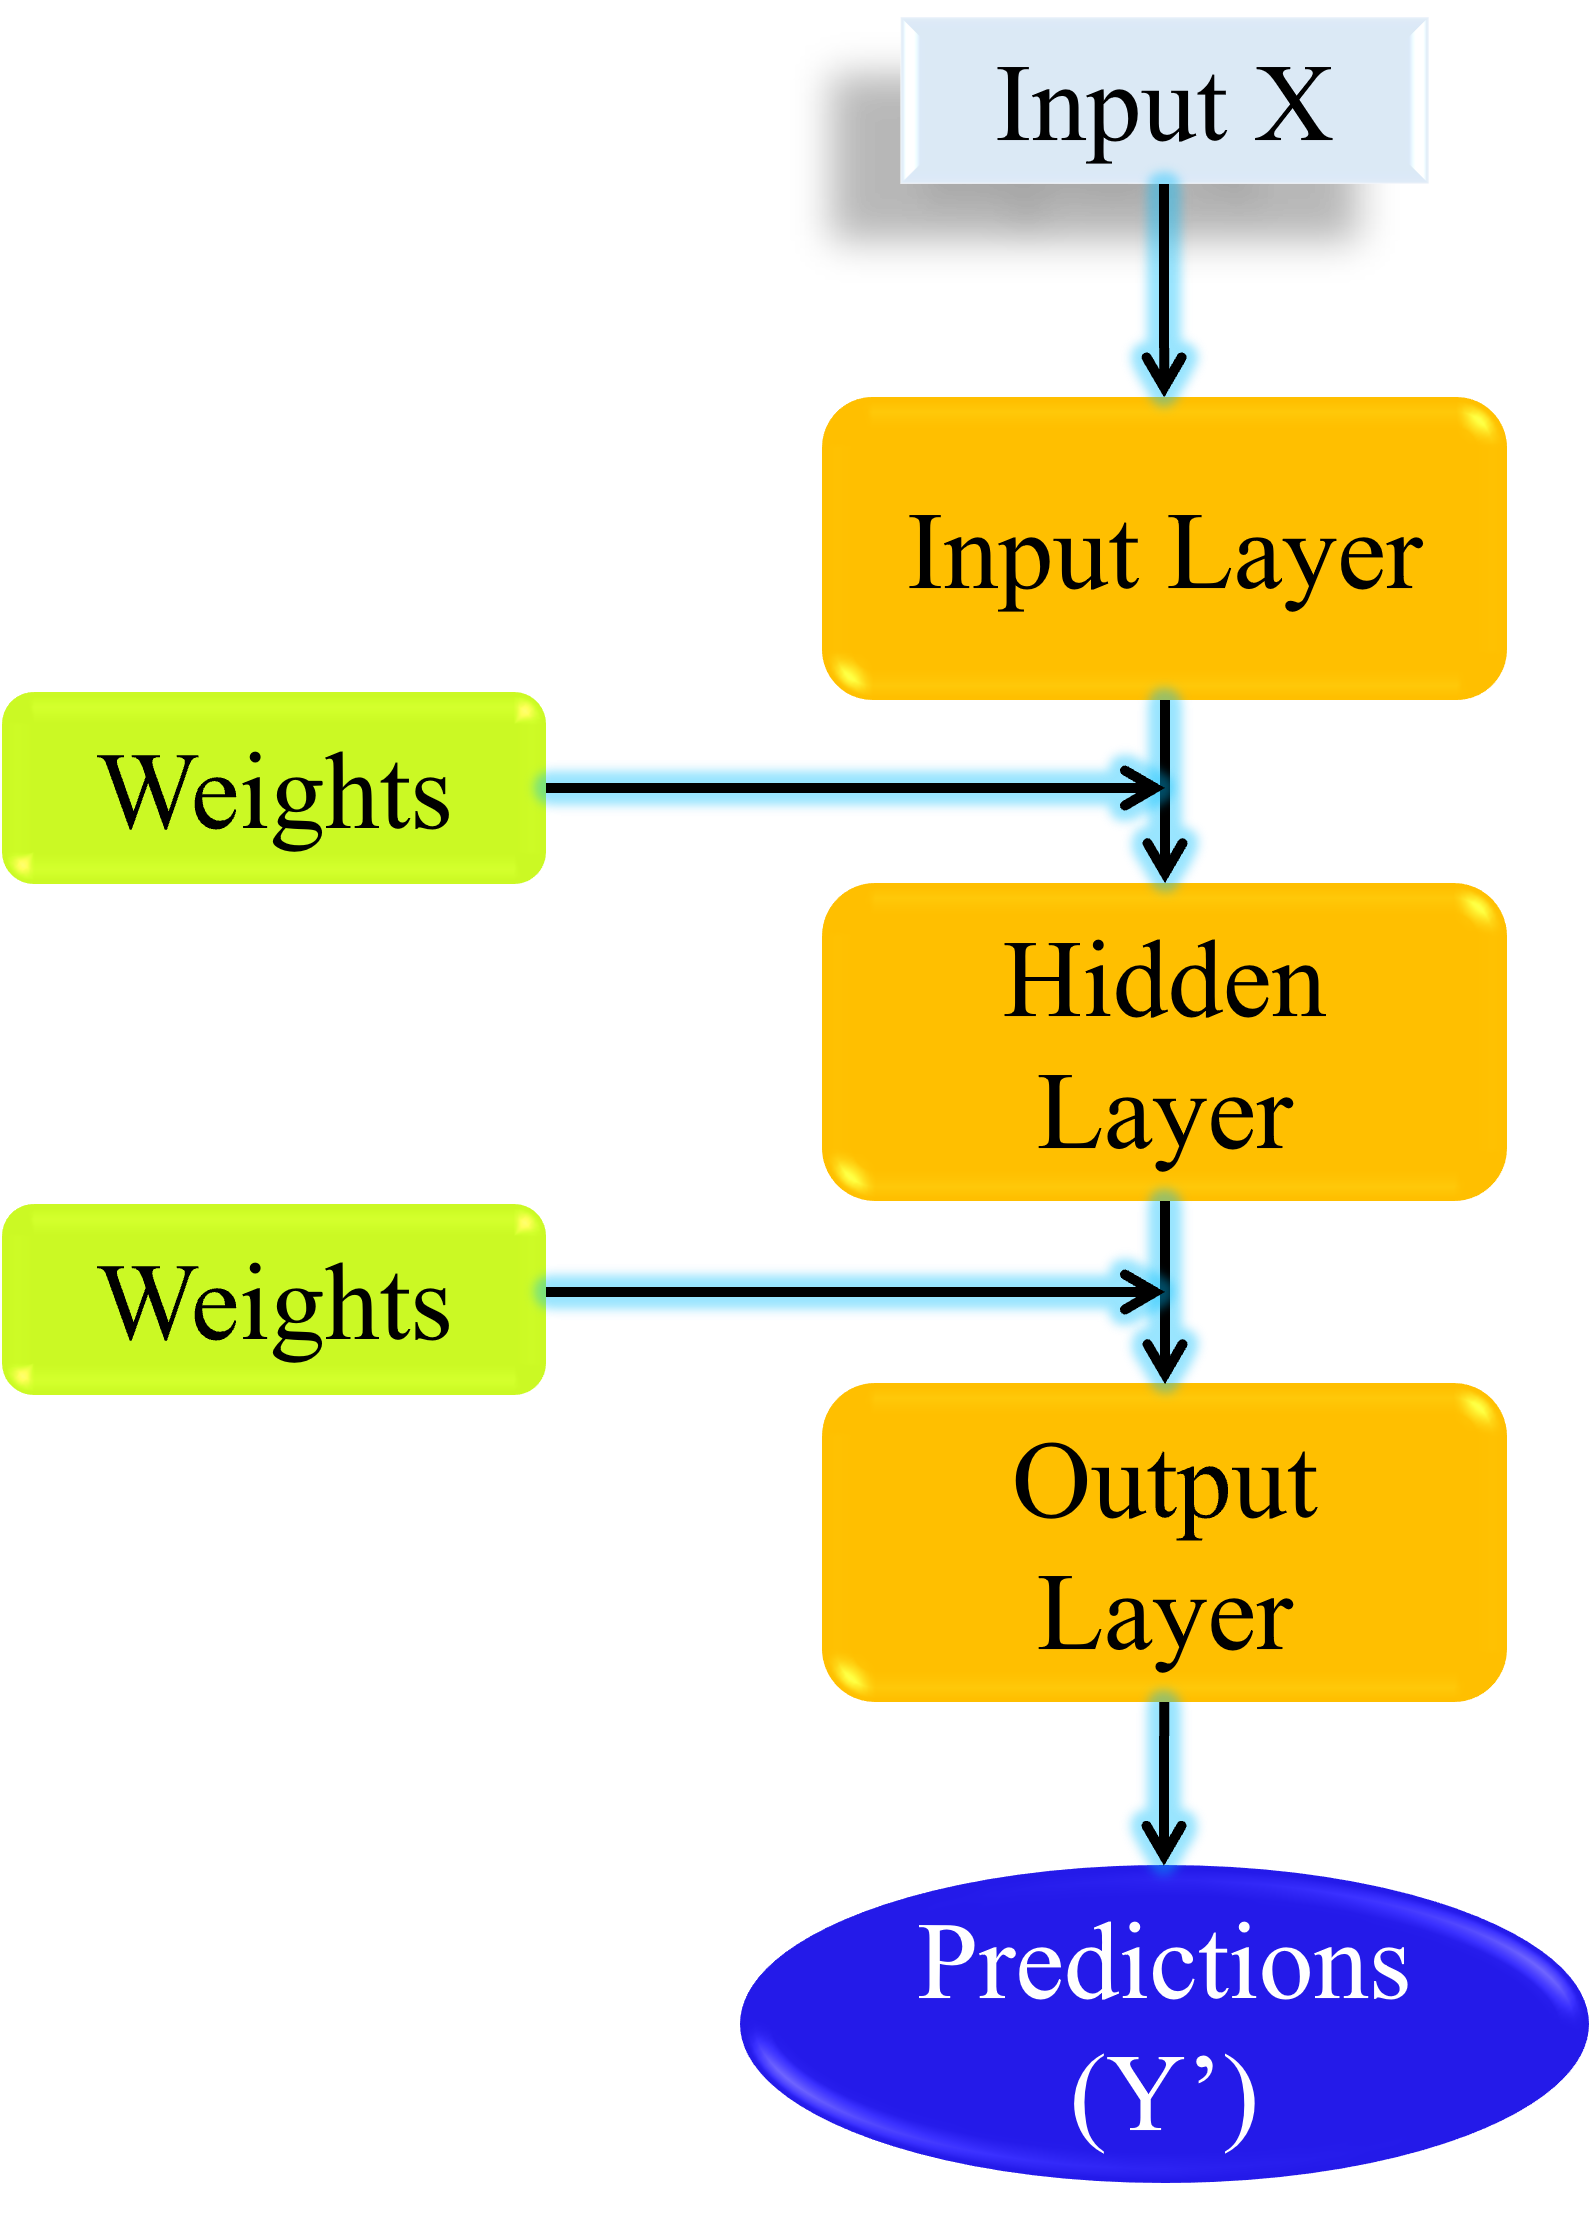
\includegraphics[width=0.4\linewidth]{images/dl_mechanism1.png}
    \caption{A deep learning model consists of a series of layers, each defined by weights that transform input data into meaningful representations.}
    \label{fig:dl_mech1}
\end{figure}
For instance, if the input to the model is rainfall intensity and the output is runoff, the first layer might perform a very basic transformation, such as amplifying the input by a random factor. Layers deeper in the model then combine these outputs into more complex patterns. The result is a series of transformations, each one building on the last, to produce the final prediction.

\subsubsection*{\textit{Loss calculation}}
To improve its predictions, the model needs a way to measure how far off its outputs are from the true values (Figure \ref{fig:dl_mech2}). This is the job of the loss function. The loss function calculates a score that represents the difference between the predicted output and the actual target. For example, if the model predicts 100 cubic meters of runoff when the actual value is 120 cubic meters, the loss function will assign a penalty to this error.
\begin{figure}[h]
    \centering
    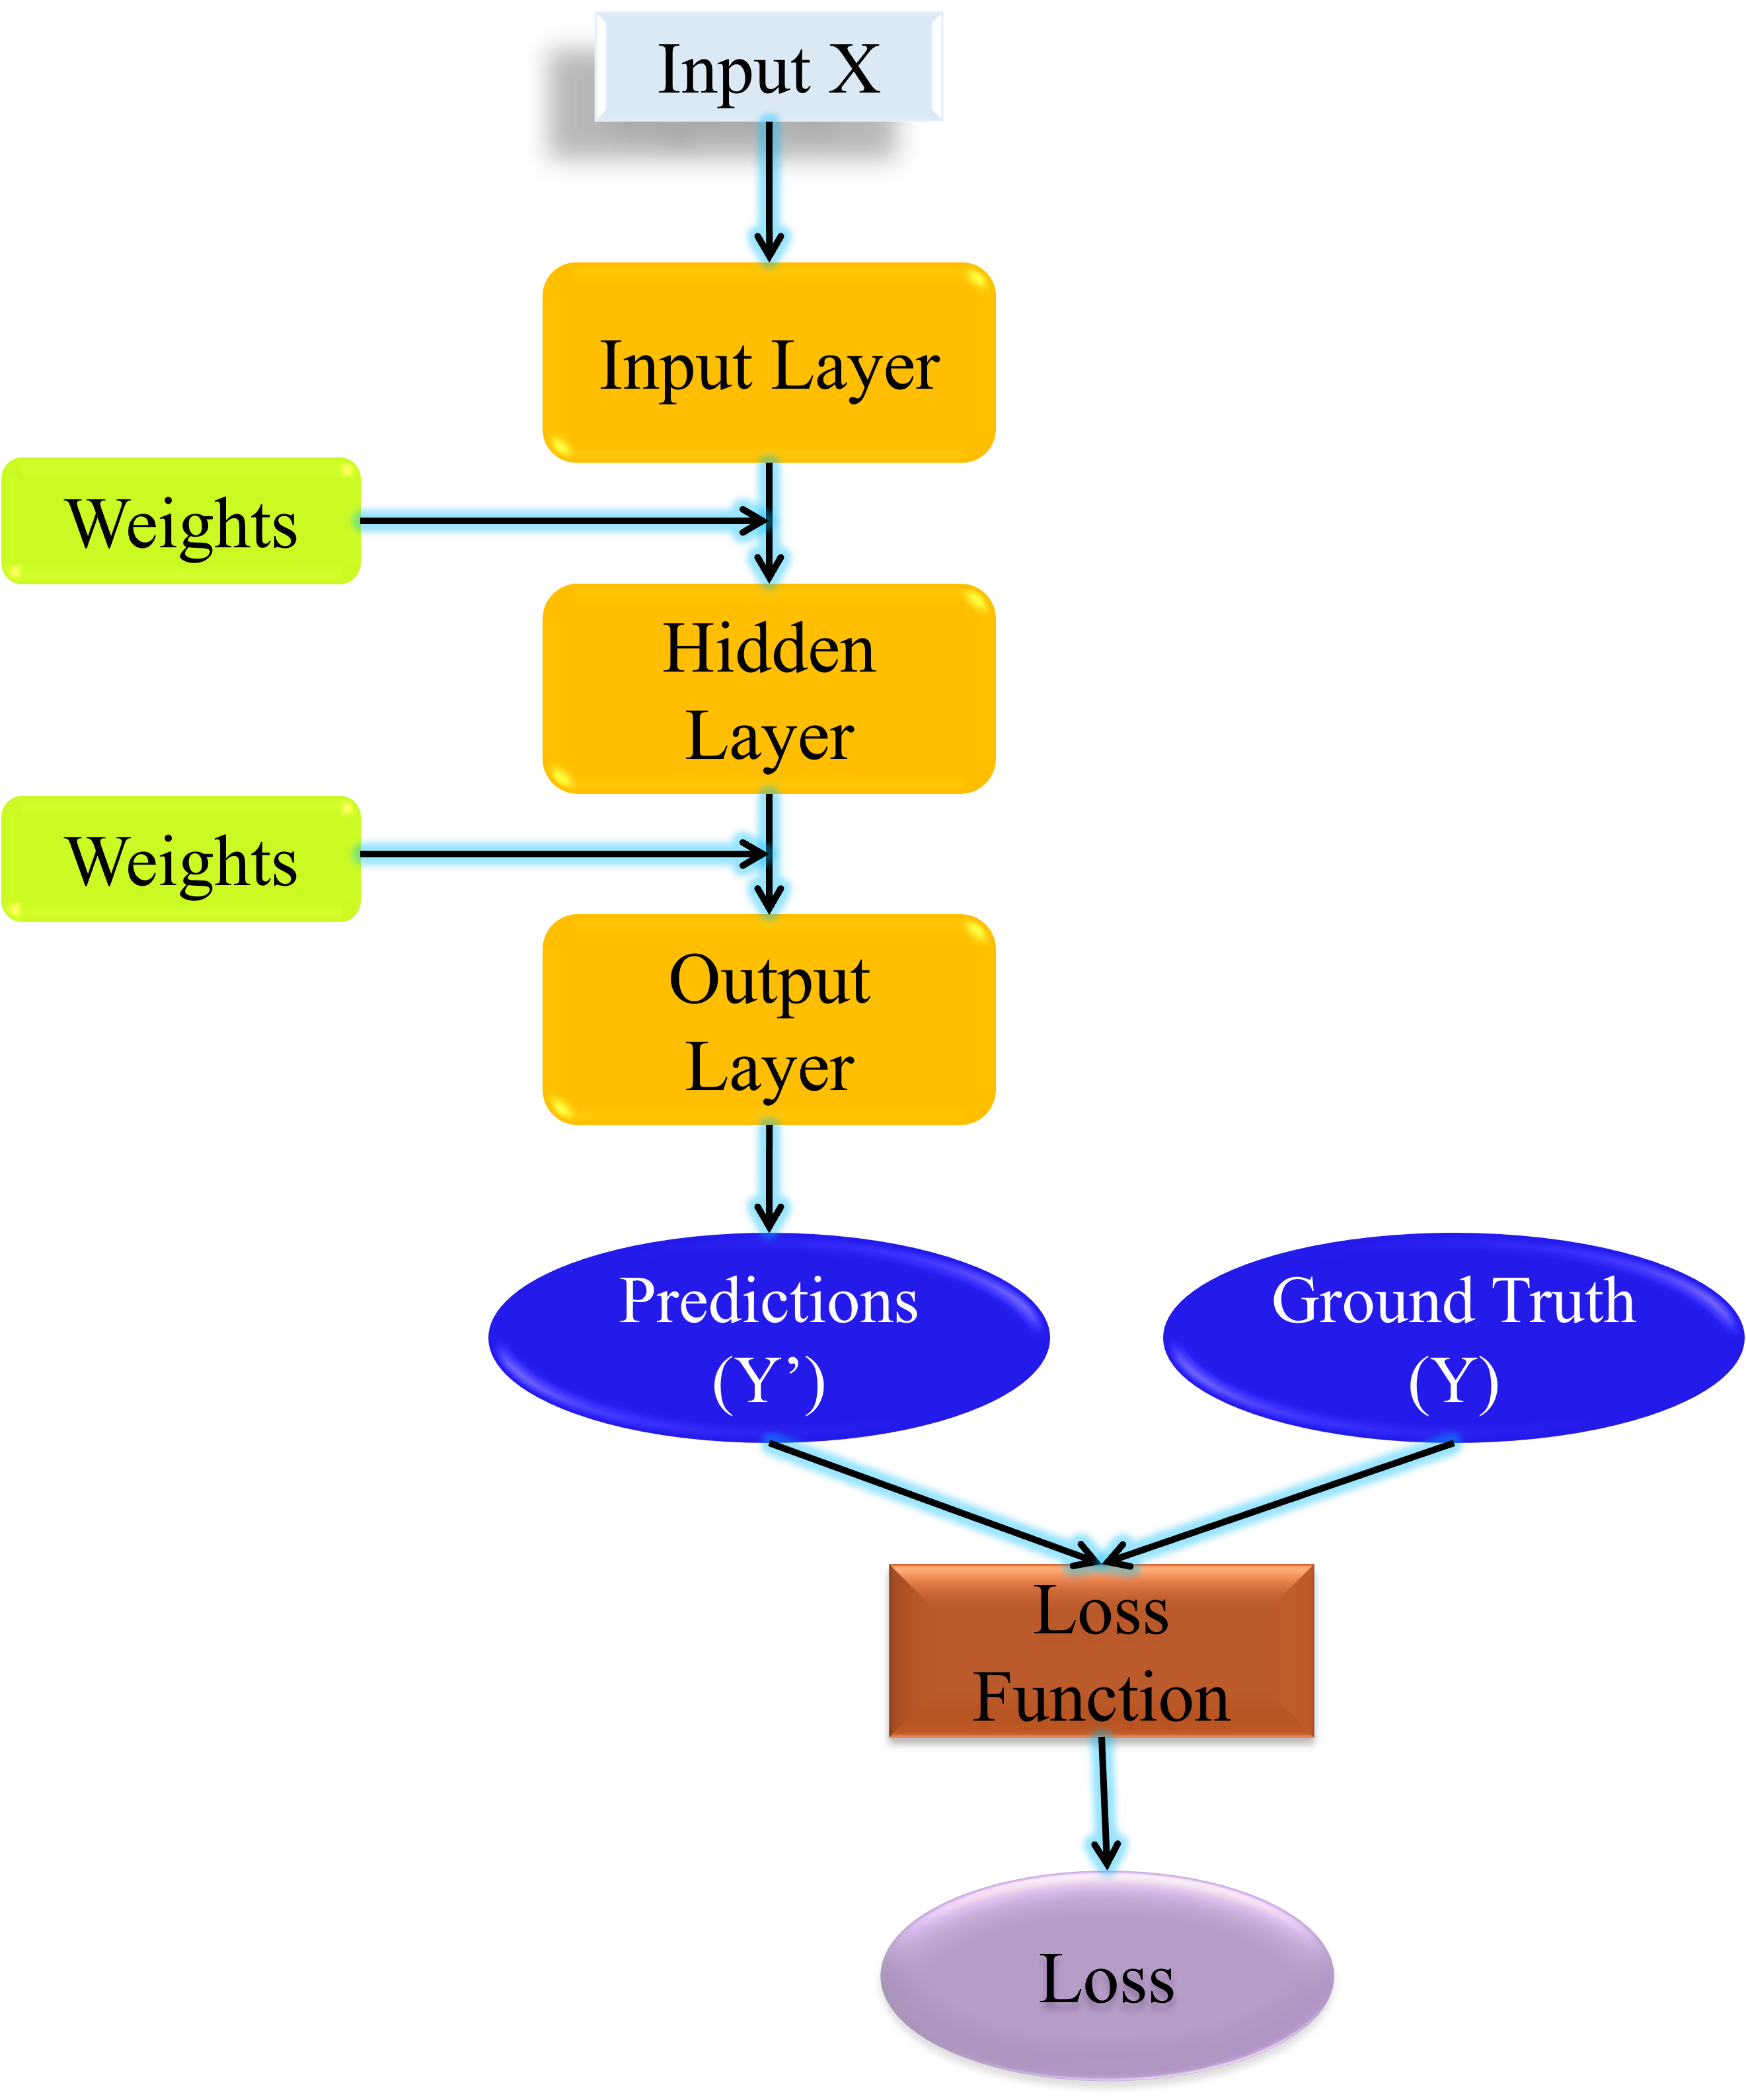
\includegraphics[width=0.4\linewidth]{images/dl_mech2.png}
    \caption{The loss function evaluates how well the model's output aligns with the target, guiding improvements through feedback.}
    \label{fig:dl_mech2}
\end{figure}
The loss function acts like a compass, pointing the model toward better predictions. The smaller the loss, the closer the model’s predictions are to the true values.
\subsubsection*{\textit{Backpropagation}} 
Once the model knows how far off it is (through the loss function), it uses this feedback to adjust its weights. This adjustment is done using an algorithm called \textit{backpropagation}, which works with an optimizer (Figure \ref{fig:dl_mech3}). The optimizer takes the loss score and calculates how each weight in the network contributed to the error. It then adjusts the weights in a way that reduces the loss.
\begin{figure}[h]
    \centering
    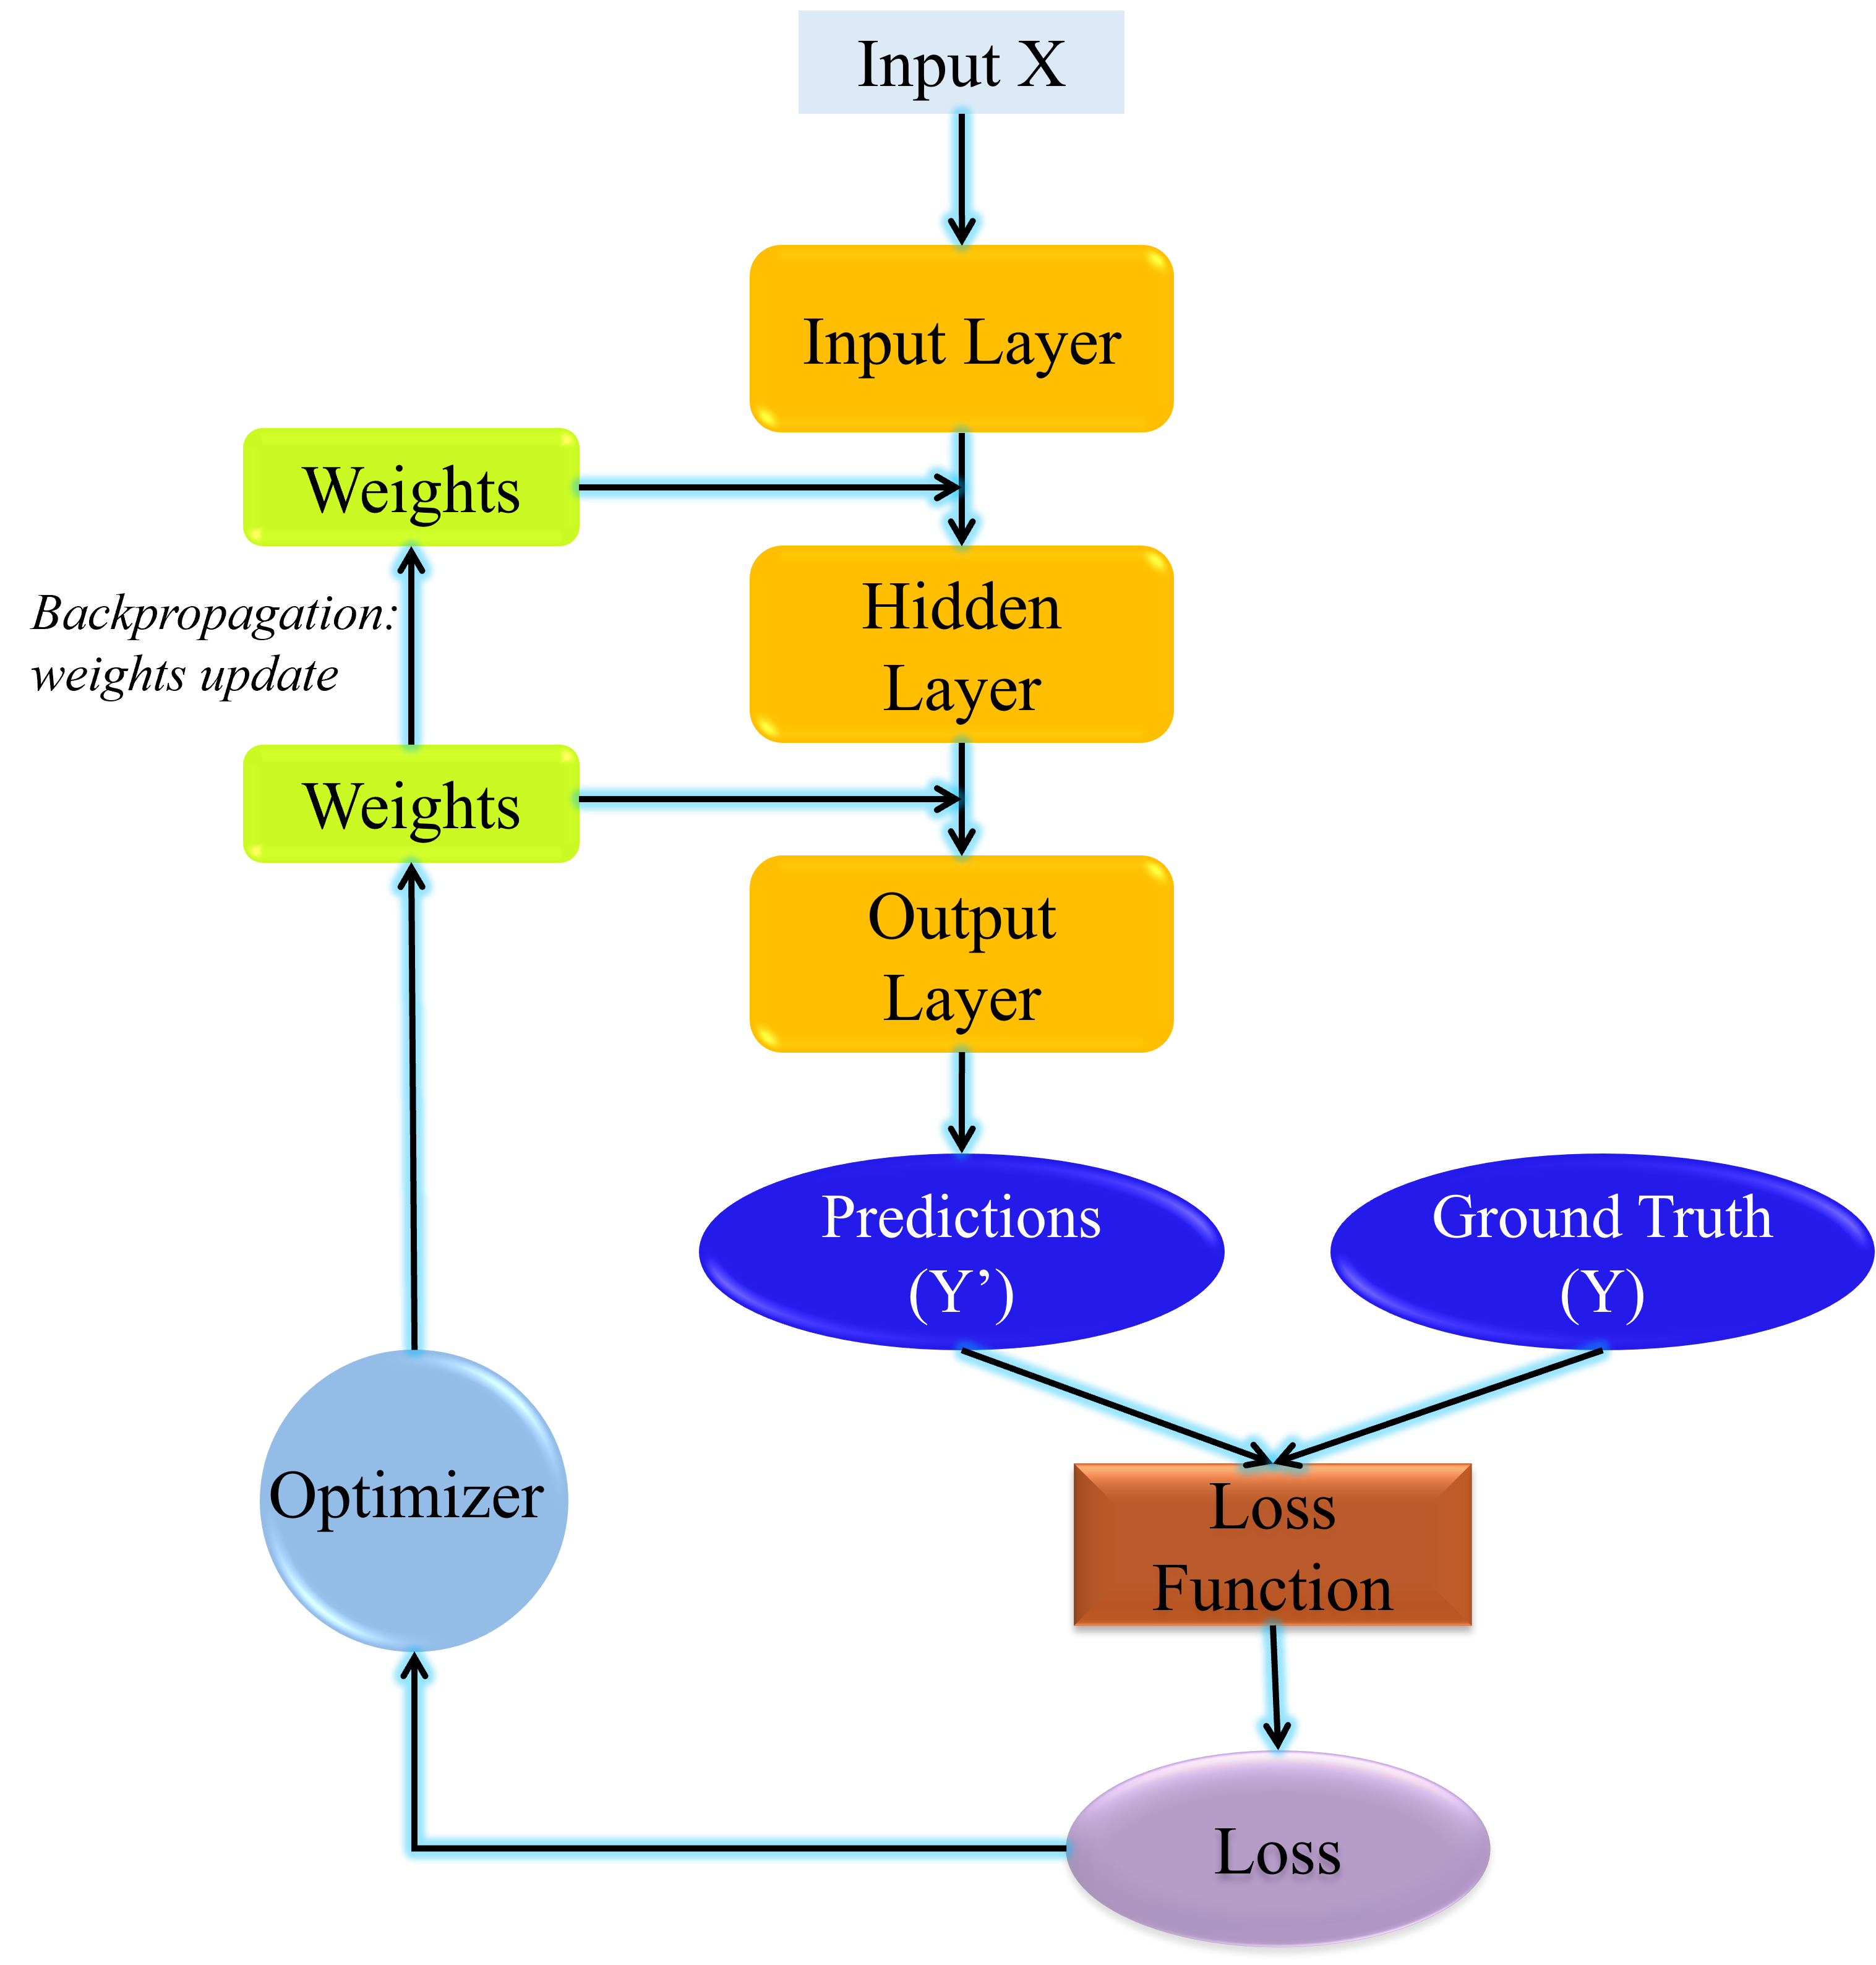
\includegraphics[width=0.7\linewidth]{images/dl_mech3.png}
    \caption{The loss score serves as feedback to adjust the model's weights through optimization and backpropagation, improving predictions with each iteration.}
    \label{fig:dl_mech3}
\end{figure}
Here’s how it works:
\begin{itemize}
    \item \textit{Prediction:} The model processes an input and produces an output using its current weights.
    \item \textit{Loss Calculation:} The loss function compares the model’s output to the true target and calculates a loss score.
    \item \textit{Backpropagation:} The optimizer calculates how to tweak each weight to reduce the loss.
    \item \textit{Parameter Update:} The weights are updated slightly in the direction that reduces the loss.
    \end{itemize}
This process is repeated for every example in the dataset, and the weights are adjusted gradually. Over time, the model’s predictions become more accurate, and the loss decreases.

\section{Regularization: Why We Need It}
As of now, you’ve learned that deep learning models can fit complex patterns in data, thanks to their multiple layers and intricate architectures. But let me ask you this: can a model be too good at fitting the data? Surprisingly, yes!

\subsubsection{\textit{The Tug-of-War Between Underfitting and Overfitting}}
instead of apples and oranges you need to explain it interms of tiug-of war also.. since we wrote that in the title.. apples and oranges are fine.. but make it better
Imagine you’re trying to teach a toddler to recognize apples and oranges. If you only tell them, “Apples are round and red,” they might struggle with oddly-shaped apples or green ones. This is underfitting—our description was too simple to capture the true variety of apples.

On the other hand, what if the toddler memorizes every single apple you showed them? They’ll recognize those apples perfectly but might fail with new ones. This is overfitting—the toddler focused too much on the examples instead of learning general rules about apples.

The same thing happens with machine learning models:

\begin{itemize}
    \item \textit{\textbf{Underfitting:}} The model is too simple to capture the patterns in the data. It performs poorly on both the training data and unseen data.
    \item \textbf{\textit{Overfitting:}} The model becomes too complex, capturing not just the patterns but also the noise in the training data. It excels on training data but fails miserably on new data.
    
\end{itemize}
So, how do we strike a balance? Enter regularization!
\subsubsection{Why Is Regularization Important?}
When training a deep learning model, we’re essentially trying to optimize its performance on unseen data. Without regularization, the model might get too attached to the training data and lose its ability to generalize. This is particularly critical in real-world scenarios, where the ultimate goal is to make accurate predictions on new, unseen data—not just the training set.

Here’s why regularization is a must:

\begin{itemize}
    \item \textbf{\textit{Generalization: }}Regularization helps ensure the model performs well on both the training data and new, unseen data.
    \item \textbf{\textit{Robustness:}} It reduces the model's sensitivity to noise in the training data, making it more stable.
    \item \textbf{\textit{Efficiency:}} A well-regularized model often requires fewer resources, as it avoids the pitfalls of complexity that don’t add value.
\end{itemize}

\subsubsection{How Does Regularization Work?}
Let’s simplify it. basically here.. we need to be consistent with the same tug-of-war example.. dont give much and different examples. stick to 1 example when explaining a concept.. dont always say imagine.. . Imagine a model as a mountain climber trying to find the lowest valley (the optimal solution). Without regularization, the climber might get stuck in every tiny dip (local patterns or noise). Regularization acts like a map, guiding the climber to avoid irrelevant dips and focus on finding the broadest, deepest valley.



As we progress through this book, you’ll come across different types of regularization techniques tailored to specific needs. 
\begin{tcolorbox}[enhanced,
  watermark opacity=0.3,watermark zoom=0.9,
  colback=blue!5!white, colframe=blue!70!white,
  fonttitle=\bfseries, title=\textit{Remember}]
  Regularization is about balance. It’s the art of making our models flexible enough to learn useful patterns but disciplined enough to avoid overfitting.
\end{tcolorbox}
\input{chapters/Part_1/DLconcepts/gradient descent}

\section{Outline:}  
Building Blocks of DL Models

Layers, weights, and activation functions.
Step-by-step walkthrough using a rainfall-runoff prediction example.
Training Deep Learning Models

Importance of loss functions and optimizers.
Concepts of overfitting and regularization techniques.
A Simple Neural Network Example

Provide a Python-based example to classify hydrological data (e.g., streamflow categories).

\section{Key Concepts in Deep Learning}
Neural Networks and Representation Learning

Introduction to tensor operations.
Role of weights and biases.
\subsection{Gradient Descent and Optimization}

Explain stochastic gradient descent.
Mention advanced optimizers (e.g., Adam, RMSProp).
Architectures in DL

Overview of CNNs, RNNs, LSTMs, and Transformers.
Application-specific suitability (e.g., CNNs for spatial data, LSTMs for time series).


\chapter{Setting the Stage: Core Mathematics of Deep Learning}
\begin{mdframed}[linewidth=1pt, linecolor=gray, backgroundcolor=gray!5] \vspace{0.2cm} \textbf{\Large After finishing this chapter, you will know:} \vspace{0.1cm}

\begin{itemize}[label=\textbf{\textendash}, leftmargin=1.5em, itemsep=0.5em, labelsep=0.5em] \item \textit{How neural networks work}: Get introduced to the structure and function of neural networks through a practical example. \item \textit{The role of tensors}: Understand tensors as the core data structures for deep learning and their representations. \item \textit{Tensor operations}: Explore foundational operations like element-wise computations, broadcasting, and reshaping, which drive neural network computations. \item \textit{How neural networks learn}: Grasp the concept of backpropagation and how optimization techniques like gradient descent enable learning. \item \textit{Connecting the dots}: See how these mathematical principles come together in a real-world example. \end{itemize} \vspace{0.2cm} \end{mdframed}


Deep learning, at its core, is about building powerful models that learn to represent and predict patterns from data. However, to truly harness its potential, you need to understand the mathematical concepts that underlie it. In this chapter, we’ll gently introduce you to these foundational ideas—without overwhelming you with unnecessary mathematical jargon.

By the end of this chapter, you’ll have a strong intuition about key mathematical building blocks like tensors, operations on tensors, and gradient-based optimization techniques. We’ll walk you through practical examples, starting with a simple neural network for a drought classification task. This example will anchor our exploration of mathematical concepts such as tensors, tensor operations, gradients, and optimization.

% \begin{enumerate}
%     \item \textbf{Introducing Neural Networks Through an Example:}We begin with a hands-on example: predicting whether a region is experiencing a drought. This practical task will introduce the fundamental ideas behind neural networks and set the stage for the deeper concepts to come.


%     \item \textbf{How Neural Networks Learn: Optimization Basics:}Dive into the mechanisms that drive learning in neural networks. We’ll explore how gradients and derivatives play a critical role in adjusting the model's parameters and introduce gradient-based optimization, including the concept of backpropagation, which powers the training process.

% \item \textbf{Putting It All Together:} After building your understanding of the core principles, we’ll revisit the drought classification example to see how these concepts work in practice. This section will reinforce your learning and prepare you for applying these ideas to real-world problems in upcoming chapters.
% \end{enumerate}
\section{Introducing Neural Networks Through a Simple Example: Drought Classification}
\section{Understanding Tensors: The Data Structures of Deep Learning}

At the heart of deep learning lies the concept of \textbf{tensors}—fundamental data structures that store and process information in neural networks. If you’ve worked with arrays or matrices before, tensors will feel familiar, as they generalize these structures to higher dimensions. Tensors are especially useful in hydrology because they can represent diverse data types across spatial, temporal, and physical dimensions.

Tensors are versatile and can handle data in various shapes and sizes, from single numbers to multidimensional arrays like images or time-series datasets. Their ability to handle multidimensional data makes them the backbone of modern deep learning frameworks like TensorFlow and PyTorch.

\subsection{What is a Tensor?}

A tensor is essentially a container for numerical data. While matrices (two-dimensional arrays) are a familiar example, tensors extend this concept to an arbitrary number of dimensions. Each tensor has three key attributes:

\begin{itemize}
    \item \textbf{Number of axes (rank):} The rank indicates how many dimensions the tensor has. For example, a scalar (single value) has no axes, a vector has one axis, and a matrix has two axes (rows and columns).
    \item \textbf{Shape:} The shape describes the number of elements along each axis. For instance, a matrix with three rows and four columns has a shape of \textit{(3, 4)}.
    \item \textbf{Data type (dtype):} This specifies the type of data stored in the tensor, such as integers (\texttt{int32}) or floating-point numbers (\texttt{float64}).
\end{itemize}

\subsection{Different Types of Tensors}
\begin{enumerate}
    \item \textbf{Scalars (0D Tensors):} Scalars are the simplest type of tensor, containing a single value with no axes.
    \begin{lstlisting}[language=Python]
    import numpy as np
    scalar = np.array(5)
    print(scalar.ndim)  # Output: 0
    \end{lstlisting}
    \textit{In hydrology, scalars might represent constants, such as the threshold for drought classification.}

    \item \textbf{Vectors (1D Tensors):} A vector is a one-dimensional array of numbers, often used to represent features of a single sample.
    \begin{lstlisting}[language=Python]
vector = np.array([45.2, 18.3, 0.35, 6.4])  # Precipitation, temp, soil moisture, evaporation
print(vector.ndim)  # Output: 1
    \end{lstlisting}
    \textit{Example: Each vector could represent features of a specific location for streamflow prediction, such as precipitation (mm), temperature (°C), soil moisture (\%), and evaporation (mm/day). A dataset with 1,000 such samples would form a 2D tensor of shape \texttt{(1000, 4)}.}

    \item \textbf{Matrices (2D Tensors):} A matrix is a two-dimensional tensor, often representing tabular datasets.
    \begin{lstlisting}[language=Python]
matrix = np.array([[1, 2, 3], [4, 5, 6], [7, 8, 9]])
print(matrix.ndim)  # Output: 2
    \end{lstlisting}
    \textit{Example: A table of daily river discharge values across multiple monitoring stations could be stored as a matrix, where rows represent days and columns represent stations.}

    \item \textbf{3D Tensors and Beyond:} Higher-dimensional tensors are created by stacking lower-dimensional tensors along new axes.
    \begin{lstlisting}[language=Python]
tensor_3d = np.array([
    [[1, 2], [3, 4]],
    [[5, 6], [7, 8]]
])
print(tensor_3d.ndim)  # Output: 3
    \end{lstlisting}
    \textit{Example: A 3D tensor might store rainfall data as grids over a region, with axes for latitude, longitude, and time. For satellite images, a 4D tensor might represent a batch of images with dimensions \texttt{(number of images, height, width, channels)}.}
\end{enumerate}

\begin{tcolorbox}[enhanced,
  watermark opacity=0.3,watermark zoom=0.9,
  colback=blue!5!white, colframe=blue!70!black,
  fonttitle=\bfseries, title=Do you know? ]
Images are often used in hydrology to represent spatial data, such as land cover, satellite images, or digital elevation models (DEMs). These are stored as 3D tensors with dimensions for height, width, and color channels.

\textbf{Flood Mapping with Satellite Images}  
\begin{itemize}
    \item  A grayscale satellite image of a flood-affected area is stored as a 3D tensor of shape \texttt{(256, 256, 1)}.
    \item  For RGB images (e.g., land cover classification), the shape becomes \texttt{(256, 256, 3)}, with three color channels (red, green, blue).
\end{itemize}

To process a batch of 100 such images, we use a 4D tensor with shape \texttt{(100, 256, 256, 3)}, where the first dimension represents the number of images.
\end{tcolorbox}



\subsection{Why Tensors Are Crucial for Hydrological Models}

Hydrological data is inherently multi-dimensional, making tensors a natural choice for data representation. Here’s why tensors are indispensable in hydrology:
\begin{itemize}
    \item \textbf{Handling Diverse Data:} Tensors allow seamless processing of both numerical vectors (e.g., precipitation and temperature) and spatial data (e.g., satellite imagery).
    \item \textbf{Capturing Spatiotemporal Relationships:} Tensors represent time-series data, spatial grids, and their interactions, enabling models to learn dependencies across time and space.
\end{itemize}


\subsection{Tensor Slicing and Indexing}

Tensors, as flexible data structures, allow for efficient manipulation through operations like slicing and indexing. These operations enable us to extract, reshape, and process relevant subsets of data. For water scientists, such operations are crucial for tasks like analyzing subsets of spatial grids, extracting temporal patterns, or managing large datasets like satellite imagery or time-series records.
Tensor slicing is a way to extract specific portions of a tensor by specifying start and end indices along each axis. This is particularly useful when working with large datasets, such as remote sensing imagery or time-series data.

\begin{itemize}
    \item \textbf{Example 1: Extracting a Subset of Remote Sensing Data}
    Consider a tensor representing a 3D satellite image of shape \texttt{(256, 256, 3)} (height, width, and RGB channels).
\begin{lstlisting}[language=Python]
import numpy as np
image = np.random.random((256, 256, 3))  # A random image
# Extract a 100x100 patch from the top-left corner
patch = image[:100, :100, :]
print(patch.shape)  # Output: (100, 100, 3)
\end{lstlisting}
You can also extract specific regions using negative indices, which count backward from the end of an axis:
\begin{lstlisting}[language=Python]
# Extract a 50x50 patch from the bottom-right corner
bottom_patch = image[-50:, -50:, :]
print(bottom_patch.shape)  # Output: (50, 50, 3)
\end{lstlisting}
\end{itemize}
\subsection{Batching Data for Training}

Deep learning models process data in batches rather than all at once. The first axis of a tensor typically represents the batch axis, where each element corresponds to one sample.
\begin{itemize}
    \item \textbf{Example 2: Preparing Batches of Rainfall Data}
    Consider a dataset of daily rainfall records for 1,000 locations over 365 days. This data can be represented as a 3D tensor of shape \texttt{(1000, 365, 1)} (locations, days, and rainfall amount):


\begin{lstlisting}[language=Python]
# Dataset with random rainfall data
rainfall_data = np.random.random((1000, 365, 1))
# Extract the first batch of 128 locations
batch = rainfall_data[:128]
print(batch.shape)  # Output: (128, 365, 1)
\end{lstlisting}
\end{itemize}

\begin{itemize}
    \item \subsubsection{Example 3: Time-Series Data}
Time-series data, such as streamflow or precipitation records, are often stored in 3D tensors with shape \texttt{(samples, features, timesteps)}, as illustrated in Figure \ref{fig:ts_3d_data}.
Suppose you have daily streamflow data (m³/s) recorded over 10 years for 100 locations. The dataset can be represented as a 3D tensor of shape \texttt{(100, 1, 3650)} (locations, streamflow, days).

\begin{figure}
    \centering
    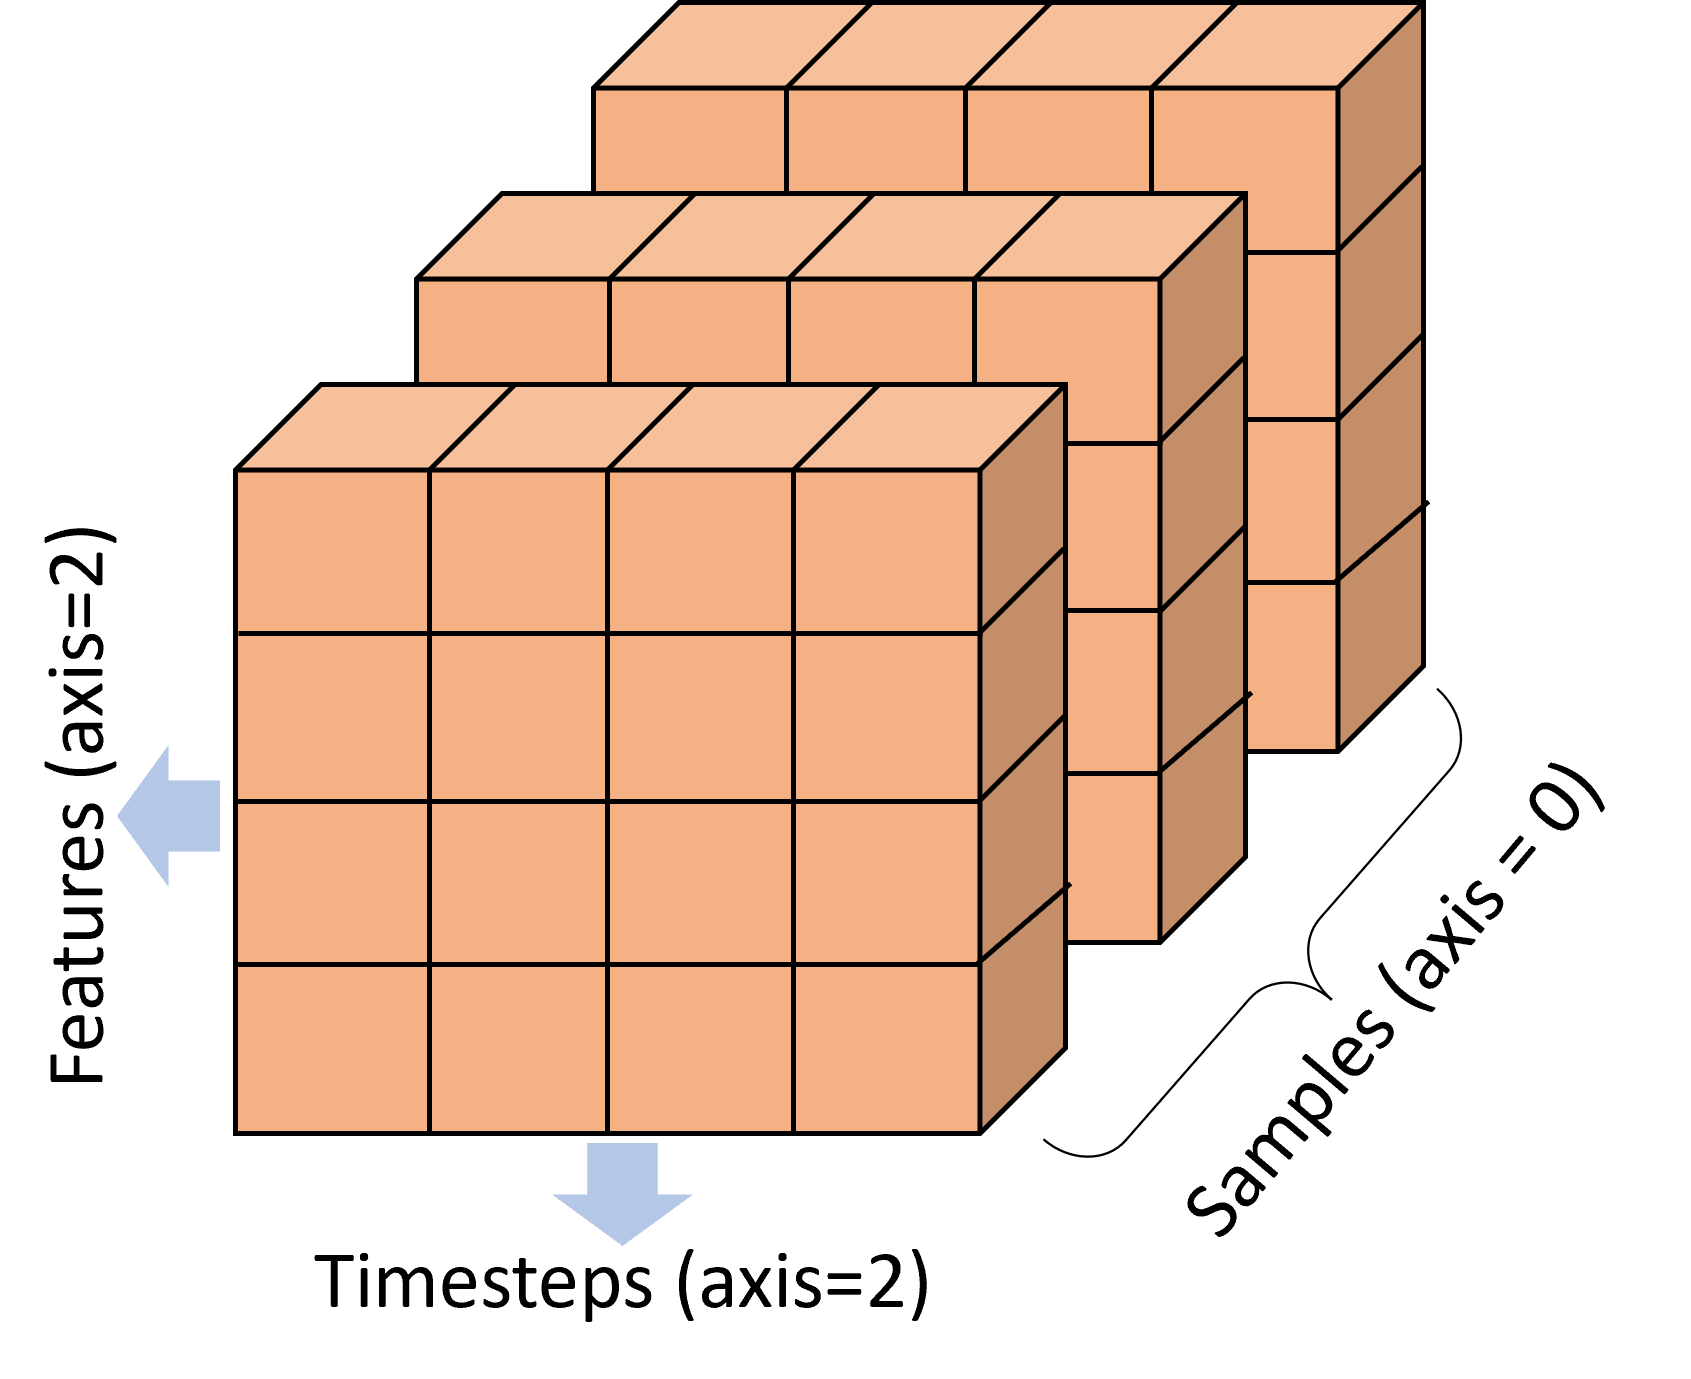
\includegraphics[width=0.5\linewidth]{images/samples-features-timesteps.png}
    \caption{Time series data represented as 3D tensors}
    \label{fig:ts_3d_data}
\end{figure}
\begin{lstlisting}[language=Python]
# Simulating streamflow data
streamflow = np.random.random((100, 1,3650))
# Extract data for the first 5 locations and the first 365 days (1 year)
subset = streamflow[:5, 0, :365]
print(subset.shape)  # Output: (5, 1, 365)
\end{lstlisting}
\end{itemize}

\begin{itemize}
    \item \subsubsection{Example 4: Satellite Image Data} 
    Satellite images are typically stored as 3D tensors (height, width, channels) or 4D tensors (batch size, height, width, channels) for a collection of images.
    In a land-cover classification example dataset of 200 satellite images, each with a resolution of 128x128 pixels and three RGB channels, would be stored as a 4D tensor of shape \texttt{(200, 128, 128, 3)}, in the format \texttt{(samples, width, height, channels)} as shown in Figure \ref{fig:4d-image-tensor}.
    \begin{lstlisting}[language=Python]
# Simulating a batch of satellite images
satellite_images = np.random.random((200, 128, 128, 3))
# Extract the first 50 images
batch_images = satellite_images[:50]
print(batch_images.shape)  # Output: (50, 128, 128, 3)
\end{lstlisting}
\end{itemize}

\begin{figure}
    \centering
    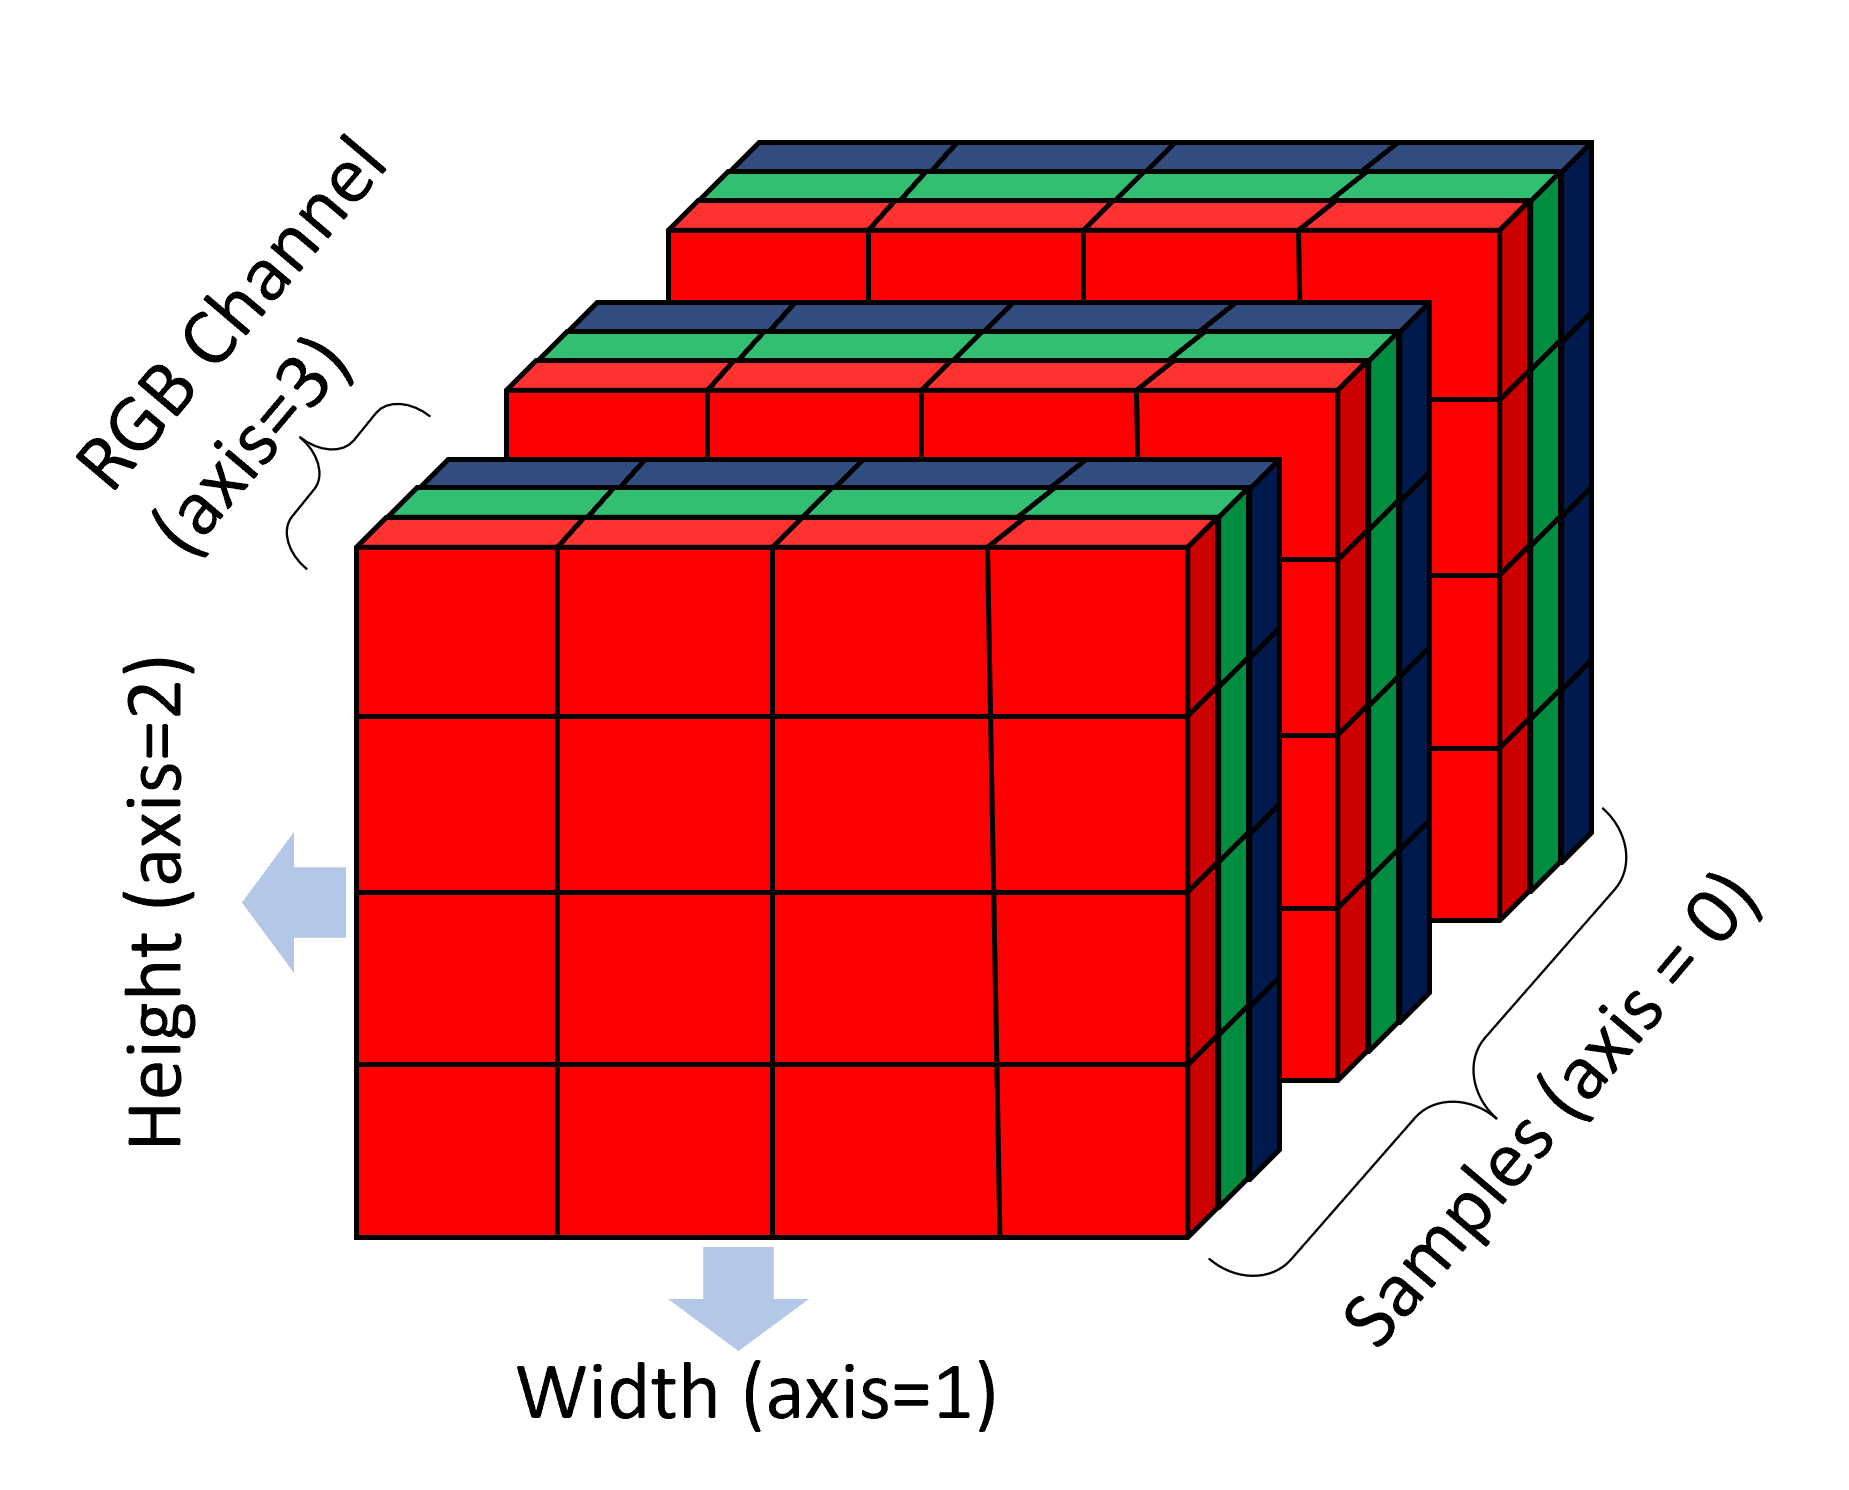
\includegraphics[width=0.5\linewidth]{images/4d-image-tensor.png}
    \caption{A 4D Image tensor data representation}
    \label{fig:4d-image-tensor}
\end{figure}





\section{Tensor Operations}


Much like computer programs are composed of simple operations on binary inputs (such as AND, OR, and XOR), deep learning models are built by applying tensor operations to numerical data. These operations are the foundation for all transformations a neural network performs. Tensor operations allow us to efficiently manipulate climate and earth science data, enabling tasks like precipitation prediction, satellite image classification, or hydrological time-series analysis.

In this section, we’ll cover the essential tensor operations—element-wise operations and broadcasting—through practical examples relevant to hydrology and remote sensing.

\subsection{Element-Wise Tensor Operations}

Element-wise operations are the simplest type of tensor operations. They involve applying a function independently to each element of a tensor or between corresponding elements of two tensors with the same shape.

\textbf{Example: Computing the Temperature Difference Between Two Grids}  
Suppose we have two temperature grids representing daily maximum and minimum temperatures (°C) over a region. These grids are stored as 2D tensors of shape \texttt{(100, 100)}, where rows and columns correspond to latitude and longitude. To compute the daily temperature range, we perform an element-wise subtraction.

\begin{lstlisting}[language=Python]
import numpy as np

# Simulated temperature grids
temp_max = np.random.random((100, 100)) * 40  # Max temperature
temp_min = np.random.random((100, 100)) * 20  # Min temperature

# Compute temperature range
temp_range = temp_max - temp_min
print(temp_range.shape)  # Output: (100, 100)
\end{lstlisting}

Each element in the \texttt{temp\_range} tensor corresponds to the temperature range at a specific grid cell.

Other common element-wise operations include addition, multiplication, and applying functions like \texttt{np.maximum()} or \texttt{np.exp()}.

---

\subsection{Broadcasting: Simplifying Operations on Tensors of Different Shapes}

In many real-world cases, tensors with different shapes need to interact. Broadcasting is a mechanism that allows smaller tensors to be automatically expanded to match the shape of larger tensors, without duplicating data in memory.

\textbf{Example: Adding a Rainfall Bias Across Multiple Regions}

Consider a dataset where daily rainfall data for 30 days is stored as a 2D tensor \texttt{rainfall} of shape \texttt{(30, 100)}, where rows represent days and columns represent regions. Suppose we want to add a constant bias correction to each region. The bias values are stored as a 1D tensor \texttt{bias} of shape \texttt{(100,)}.

\begin{lstlisting}[language=Python]
# Simulated rainfall data (mm) and bias correction
rainfall = np.random.random((30, 100)) * 50  # Daily rainfall
bias = np.random.random((100,)) * 2          # Bias for each region

# Add bias using broadcasting
corrected_rainfall = rainfall + bias
print(corrected_rainfall.shape)  # Output: (30, 100)
\end{lstlisting}

\textbf{How Broadcasting Works:}
1. The \texttt{bias} tensor of shape \texttt{(100,)} is reshaped to \texttt{(1, 100)} by adding a new axis.
2. The reshaped \texttt{bias} tensor is virtually repeated 30 times along the first axis to match the shape of \texttt{rainfall} (\texttt{(30, 100)}).
3. Element-wise addition is performed between the tensors.

\textit{Note:} Broadcasting happens at the algorithmic level and does not physically create new tensors, ensuring memory efficiency.

---

\subsubsection{A Practical Example in Remote Sensing}

Let’s consider satellite images with shape \texttt{(64, 3, 128, 128)}, representing a batch of 64 images with 3 color channels (RGB) and dimensions 128x128 pixels. We wish to normalize each pixel intensity by subtracting the mean intensity of its channel.

\begin{lstlisting}[language=Python]
# Simulated batch of images
images = np.random.random((64, 3, 128, 128)) * 255

# Mean intensity per channel
channel_mean = images.mean(axis=(0, 2, 3), keepdims=True)

# Normalize using broadcasting
normalized_images = images - channel_mean
print(normalized_images.shape)  # Output: (64, 3, 128, 128)
\end{lstlisting}

Here, the mean tensor \texttt{channel\_mean} is broadcasted to match the shape of \texttt{images}, enabling efficient subtraction across all pixels.

---

\subsection{Why Tensor Operations Matter in Hydrology}

Tensor operations are essential for:
\begin{itemize}
    \item \textbf{Analyzing Spatial Data:} Compute statistics, such as temperature ranges or precipitation anomalies, over grids.
    \item \textbf{Normalizing Datasets:} Prepare remote sensing images or time-series data for model training.
    \item \textbf{Efficient Computation:} Perform complex operations on large datasets without duplicating memory.
\end{itemize}

These operations are the building blocks for designing and training deep learning models tailored to hydrology and earth sciences.


\section{How Neural Networks Learn: Optimization Basics}


\chapter{Fundamentals of Deep Learning}



% ---------------------------------------- Major Branches of Deep Learning -------------------------
\section{Major Branches of Deep Learning}
\subsection{Supervised Learning}
Supervised learning is one of the most widely used branches of deep learning. It involves training models on datasets where each input is paired with a corresponding output, commonly referred to as a \textit{label}. This approach enables models to learn the relationship between inputs and their known results, allowing them to make accurate predictions on new, unseen data. In essence, supervised learning is like teaching a system through examples where the correct answers are already provided.
Supervised learning tasks typically fall into two categories:
\begin{itemize}
\item \textit{Classification:} Sorting data into predefined categories. For example, classifying land cover types (e.g., forests, urban areas, water bodies) based on satellite images.
\item \textit{Regression:} Predicting continuous numerical values. An example is forecasting river water levels based on historical data and environmental conditions.
\end{itemize}
Supervised learning () plays a pivotal role in hydrology and environmental sciences, powering a wide range of applications such as image classification, temperature forecasting, and hurricane tracking. To tackle these tasks, specific deep learning architectures are particularly effective. For example, Recurrent Neural Networks (RNNs) and their advanced variant, Long Short-Term Memory networks (LSTMs), excel at processing and forecasting sequential data, making them ideal for analyzing time-series datasets like rainfall records or river flow patterns. On the other hand, Convolutional Neural Networks (CNNs) are exceptionally adept at handling image-based tasks. They are commonly used for interpreting satellite images, such as identifying land cover types or detecting environmental changes.
Here are some representative examples of how supervised learning is applied in hydrology and environmental sciences:
\begin{itemize}
    \item \textit{Precipitation Forecasting:} Predicting rainfall amounts to aid in water resource management and flood prevention.
\item \textit{Drought Severity Classification:} Determining the severity of droughts to assist in agricultural planning and water conservation.
\item \textit{Land Cover Classification:} Categorizing earth surface types (e.g., forests, croplands, urban areas) from satellite imagery for applications like urban planning and ecosystem monitoring.
\item \textit{Image Segmentation:} Identifying specific regions in satellite images, such as flood-affected areas, deforested zones, or crop health conditions.
\item \textit{Object Detection:} Identifying and categorizing objects in satellite imagery, such as water bodies, vegetation types, or urban areas.
\end{itemize}


\begin{figure}[h!]
    \centering
    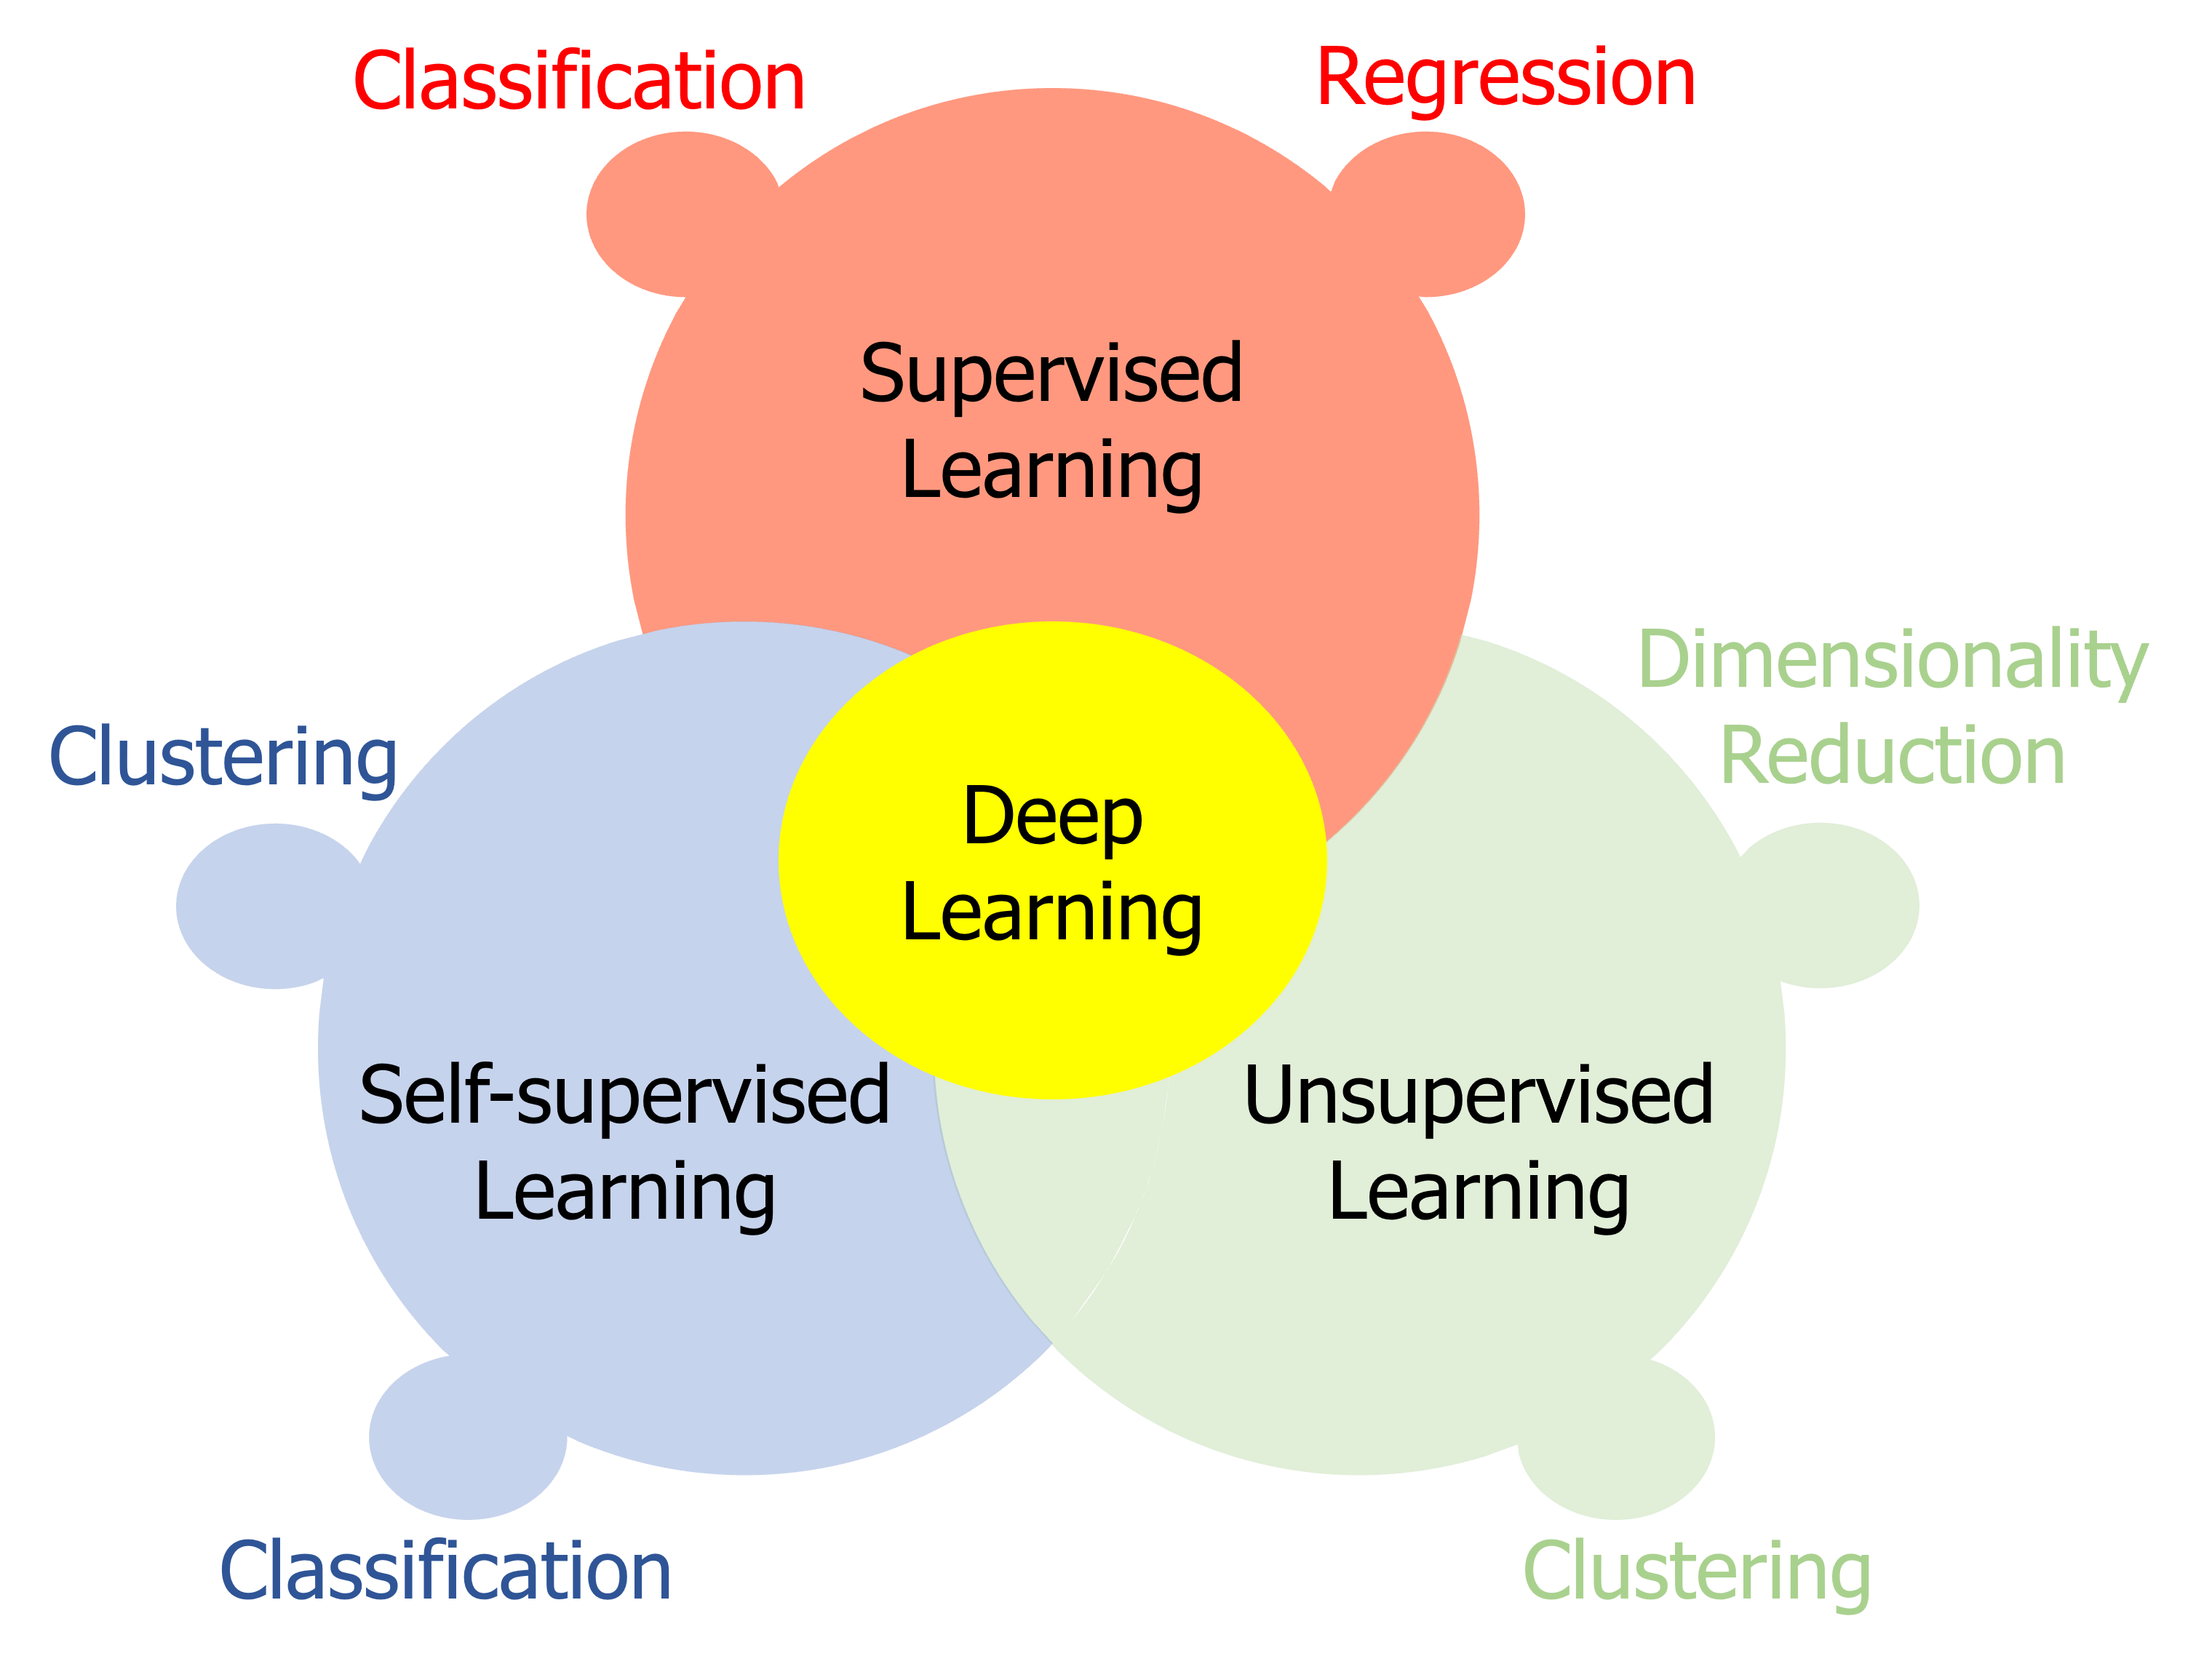
\includegraphics[width=\linewidth]{images/supervised_learning_classification_image.png}
    \caption{Three Major branches of Deep Learning: supervised learning, unsupervised learning, and self-supervised learning.}
    \label{fig:supervised}
\end{figure}


\subsection{Unsupervised Learning }

Unsupervised learning focuses on uncovering patterns, structures, and transformations within data, all without relying on labeled outputs. Instead of predicting a specific target, it aims to reveal insights such as correlations, clusters, or low-dimensional representations. This type of learning is invaluable in hydrology and environmental sciences, where complex datasets often need to be distilled into more interpretable or actionable forms. 
Unsupervised learning is foundational for tasks like data visualization, where the goal is to represent high-dimensional data in an intuitive way, and dimensionality reduction, which simplifies large datasets while retaining essential information. It also plays a critical role in data denoising, improving the quality of noisy remote sensing data to make subsequent analyses more reliable. Before solving supervised learning problems, unsupervised learning can act as a crucial first step to explore and understand the dataset, identify outliers, and discover hidden relationships.

\begin{itemize}
    \item \textit{Data Visualization:} Creating intuitive visual representations of high-dimensional datasets, such as water quality measurements spanning multiple variables, to better understand spatial and temporal trends.
    \item \textit{Dimensionality Reduction:} Simplifying vast climatic datasets, like global temperature records or precipitation grids, for faster processing and storage while preserving critical patterns.
    \item \textit{Data Denoising:} Enhancing the quality of noisy remote sensing data (e.g., satellite imagery or LiDAR scans) to improve the accuracy of downstream analyses like land cover classification or flood mapping.
    \item \textit{Clustering:} Identifying groups in the data, such as categorizing regions based on similar hydrological characteristics or climate patterns, without pre-defined labels.

\end{itemize}


\subsection{Self-Supervised Learning}

Self-supervised learning is a DL approach where the model generates its own labels directly from the input data, removing the need for human-annotated labels. These pseudo-labels guide the learning process, making it possible to utilize large amounts of unlabeled data. This is particularly beneficial in hydrology, where labeled datasets are often limited or incomplete.

A key advantage of self-supervised learning is its scalability. By automatically generating pseudo-labels, it avoids the time and cost associated with manual labeling. A well-known example of self-supervised learning is the autoencoder, a model that compresses data into a compact representation (the "encoder") and then reconstructs it back to its original form (the "decoder"). The reconstruction error—the difference between the input and the reconstructed output—provides the learning signal. We will explore autoencoders in detail in Chapter~\ref{chap:acn} with a practical example.

Here are two simple examples to illustrate self-supervised learning:

\begin{itemize}
    \item \textit{Noise Removal in Satellite Images:} Autoencoders can clean noisy satellite images by learning to reconstruct meaningful features, such as water boundaries, while removing noise.
    \item \textit{Predicting Missing Data:} Models can predict missing streamflow values based on surrounding data, helping to fill gaps in hydrological records for further analysis.
\end{itemize}

\textbf{NOTE:} In this book, we’ll primarily focus on supervised learning, as it remains the most widely used and impactful form of deep learning in hydrology and environmental sciences, powering applications like precipitation forecasting, flood mapping, and drought prediction. We’ll also briefly explore self-supervised learning in later chapters, as it offers promising solutions for leveraging large, unlabeled datasets, which are common in these fields.

\subsection{Reinforcement Learning (RL)}
There is another branch of DL called Reinforcement Learning (RL), where an agent interacts with its environment, learning through trial and error to take actions that maximize a reward signal. Unlike traditional DL, which focuses on mapping inputs to outputs, RL emphasizes decision-making in dynamic environments. For example, an RL model could determine optimal reservoir release strategies by balancing flood control and water conservation. While RL has shown success in fields like robotics and gaming, its applications in hydrology are still largely in the research phase. In this book, we will primarily focus on supervised learning, leaving RL for further exploration in advanced studies.

% ----------------------------------------Evaluating Deep Learning Models -------------------------




























\section{Evaluating Deep Learning Models}
Understanding how to evaluate deep learning models effectively is crucial for developing robust neural networks.

\subsection{Data Splits: Training, Validation, and Test Sets}
To evaluate a model, we divide our dataset into three distinct sets:

\begin{enumerate}
    \item \textit{Training Set:} Used to train the model. The model learns patterns and adjusts its parameters on this data.
    \item \textit{Validation Set}: Used to tune the model’s hyperparameters, such as the number of layers or learning rate. It acts as a feedback mechanism to guide model improvements without being part of training.
    \item \textit{Test Set:} Used to assess the model’s final performance. It represents completely unseen data and ensures that the model generalizes well beyond the data it was trained or validated on.
\end{enumerate}

\paragraph{Why Not Just Use Two Sets? \newline}

At first glance, splitting the data into only training and test sets might seem simpler. However, developing a model often involves hyperparameter tuning, where decisions about the model’s architecture or training process are made based on its performance during development. Relying only on the test set for this tuning can lead to \textit{information leaks}, where the test data indirectly influences the model. This results in overly optimistic evaluations that don’t reflect real-world performance. The validation set prevents this by acting as an intermediate checkpoint. The test set is kept untouched until the very end, ensuring a fair assessment.

\paragraph{The Risk of Overfitting the Validation Set\newline}

Repeatedly tuning a model based on validation performance can inadvertently make the model overly specialized to the validation data. This happens because small amounts of information about the validation set "leak" into the model during each tuning step. If this process is repeated many times, the validation set’s reliability as an unbiased evaluation metric diminishes. To ensure a truly robust evaluation, the test set must remain untouched throughout the development process.


% --------------------------------- Overfitting, Underfitting, and Model Optimization ---------------

\section{Overfitting, Underfitting, and Model Optimization}
\label{sc:overfitting}
In the previous examples—temperature forecasting, classifying drought severity, and modeling lake water temperatures—we observed a common trend: the performance of the model on held-out validation data often peaked after a few training epochs and then began to degrade. This phenomenon, where a model performs well on training data but poorly on unseen data, is known as \textit{overfitting}. Overfitting is a challenge faced in every deep learning project, and mastering strategies to combat it is crucial for building effective models.
At the heart of this challenge is the tension between \textbf{optimization} and \textbf{generalization}:
Optimization refers to the process of training a model to perform as well as possible on the training data. Essentially, this is the \textit{learning} in DL. Generalization, on the other hand, is the ability of the trained model to perform well on unseen data.
Our ultimate goal is to achieve good generalization. However, generalization cannot be directly controlled during training; we can only adjust the model based on its performance on the training data. Understanding this balance is key to building robust models for hydrology and environmental sciences.
At the beginning of training, optimization and generalization are typically aligned: as the model's performance on the training data improves, so does its performance on validation data. During this stage, the model is said to be \textit{underfitting}. Underfitting occurs when the model has not yet captured all the relevant patterns in the training data, leaving room for improvement.

However, after a certain number of training iterations, a turning point is reached where the performance on the validation data stops improving. Beyond this point, continued optimization on the training data causes the model to overfit. \textit{Overfitting occurs when the model begins to memorize patterns that are specific to the training data} rather than learning generalizable patterns. These irrelevant patterns do not translate well to unseen data, leading to degraded performance on the validation set.

The most effective way to prevent overfitting is to \textit{increase the amount of training data}. With more diverse and representative data, the model can naturally generalize better to unseen examples. However, in many cases—especially in hydrology and environmental sciences—collecting additional data can be costly, time-consuming, or even impossible due to physical and logistical constraints.
When more data is not an option, the next-best approach is to restrict the amount of information the model can store or impose constraints on how it learns. This ensures the model focuses on the most relevant patterns in the data, which are more likely to generalize well. Techniques that achieve this are collectively referred to as \textbf{regularization}, which are discussed in section \ref{sc:reg}.


Regularization introduces constraints that limit a model's capacity to memorize irrelevant patterns, helping it generalize better. The underlying idea is simple: if a model can only "afford" to store a limited number of patterns, it will prioritize learning the most prominent and meaningful ones. Regularization methods include:


In the next section, we will explore these regularization techniques in detail and demonstrate how to apply them to improve the performance of a precipitation classification model.







\subsection{Weight Regularization}
\subsection{Early Stopping}
Early stopping is another effective technique for avoiding overfitting. It monitors the model’s performance on a validation set during training and stops training when performance on the validation set stops improving. This prevents the model from continuing to train and overfit the training data.

For example, a DL model might overfit after 100 epochs even though validation performance peaked at 50 epochs (\ref{fig:earlystop}). Early stopping stops the training process automatically, saving time and ensuring the best-performing model is retained.
In Keras, early stopping is implemented using the \textit{EarlyStopping} callback. For example:

\begin{lstlisting}[language=Python]
from keras.callbacks import EarlyStopping

# Define an EarlyStopping callback
early_stopping = EarlyStopping(monitor='val_loss', patience=5, restore_best_weights=True)

# Train the model 
model.fit(X_train, y_train, validation_data=(X_val, y_val), epochs=100, callbacks=[early_stopping])

\end{lstlisting}
Here:
\begin{itemize}
    \item \texttt{monitor= 'val\_loss'} tracks the validation loss.
    \item patience=5 means training stops if validation loss does not improve for 5 consecutive epochs.
    \item \texttt{restore\_best\_weights=True} ensures the best model is saved.
\end{itemize}

\subsection{Dropout Regularization}
Dropout is a simple yet powerful technique where a fraction of neurons in a layer is randomly "dropped out" during each training step. These dropped-out neurons do not contribute to the forward pass or the backward pass (gradient updates). This forces the network to learn more robust features by ensuring that no single neuron or group of neurons becomes overly specialized or reliant on specific connections.

For example, imagine a network that predicts runoff based on rainfall, temperature, and soil moisture. If some neurons are randomly deactivated during training, the network must learn alternative pathways and redundant features, improving its ability to generalize.

Key points about dropout:

\begin{itemize}
    \item Dropout is applied only during training, not during testing.
    \item The dropout rate specifies the fraction of neurons to drop (typically between 0.2 and 0.5).
    \item It works like training an ensemble of smaller subnetworks, which combine into a stronger overall model.
\end{itemize}
Adding dropout to a model in Keras is straightforward. For example:
\begin{lstlisting}[language=Python]
from keras.models import Sequential
from keras.layers import Dense, Dropout
# Define a model with dropout
model = Sequential([
    Dense(64, activation='relu', input_shape=(10,)),  # Input layer
    Dropout(0.3),  # Dropout layer with 30% rate
    Dense(32, activation='relu'),
    Dropout(0.2),  # Dropout layer with 20% rate
    Dense(1, activation='sigmoid')  # Output layer])
model.compile(optimizer='adam', loss='binary_crossentropy', metrics=['accuracy'])
\end{lstlisting}
\subsection{Batch Normalization}
\subsection{K-fold Cross-Validation}
K-fold cross-validation is a practical technique to evaluate model performance and reduce overfitting (discussed in detail in section \ref{sc:overfitting}), especially when data is limited. It works by dividing the dataset into k equal parts, called folds. For instance, if \textit{k=4}, the data is split into 4 subsets (Figure \ref{fig:kfold}). The model is trained on 3 folds and validated on the 1 remaining fold. This process is repeated 4 times, so each fold serves as the validation set exactly once. The final performance is averaged across all 4 runs, providing a robust estimate of the model's ability to generalize to new data.

This method ensures that all data points are used for both training and validation, making the most of limited datasets. For example, if the data is not shuffled before splitting, similar types of data (e.g., seasonal trends in hydrological data) might cluster in one fold, leading to biased results. By shuffling the data beforehand, each fold becomes more representative of the entire dataset, improving the reliability of the evaluation.

K-fold cross-validation is essential because it reduces the risk of overfitting. It ensures the model is tested on different subsets of data, exposing it to various patterns and reducing dependency on any single data split.



\begin{figure}[h!]
    \centering
    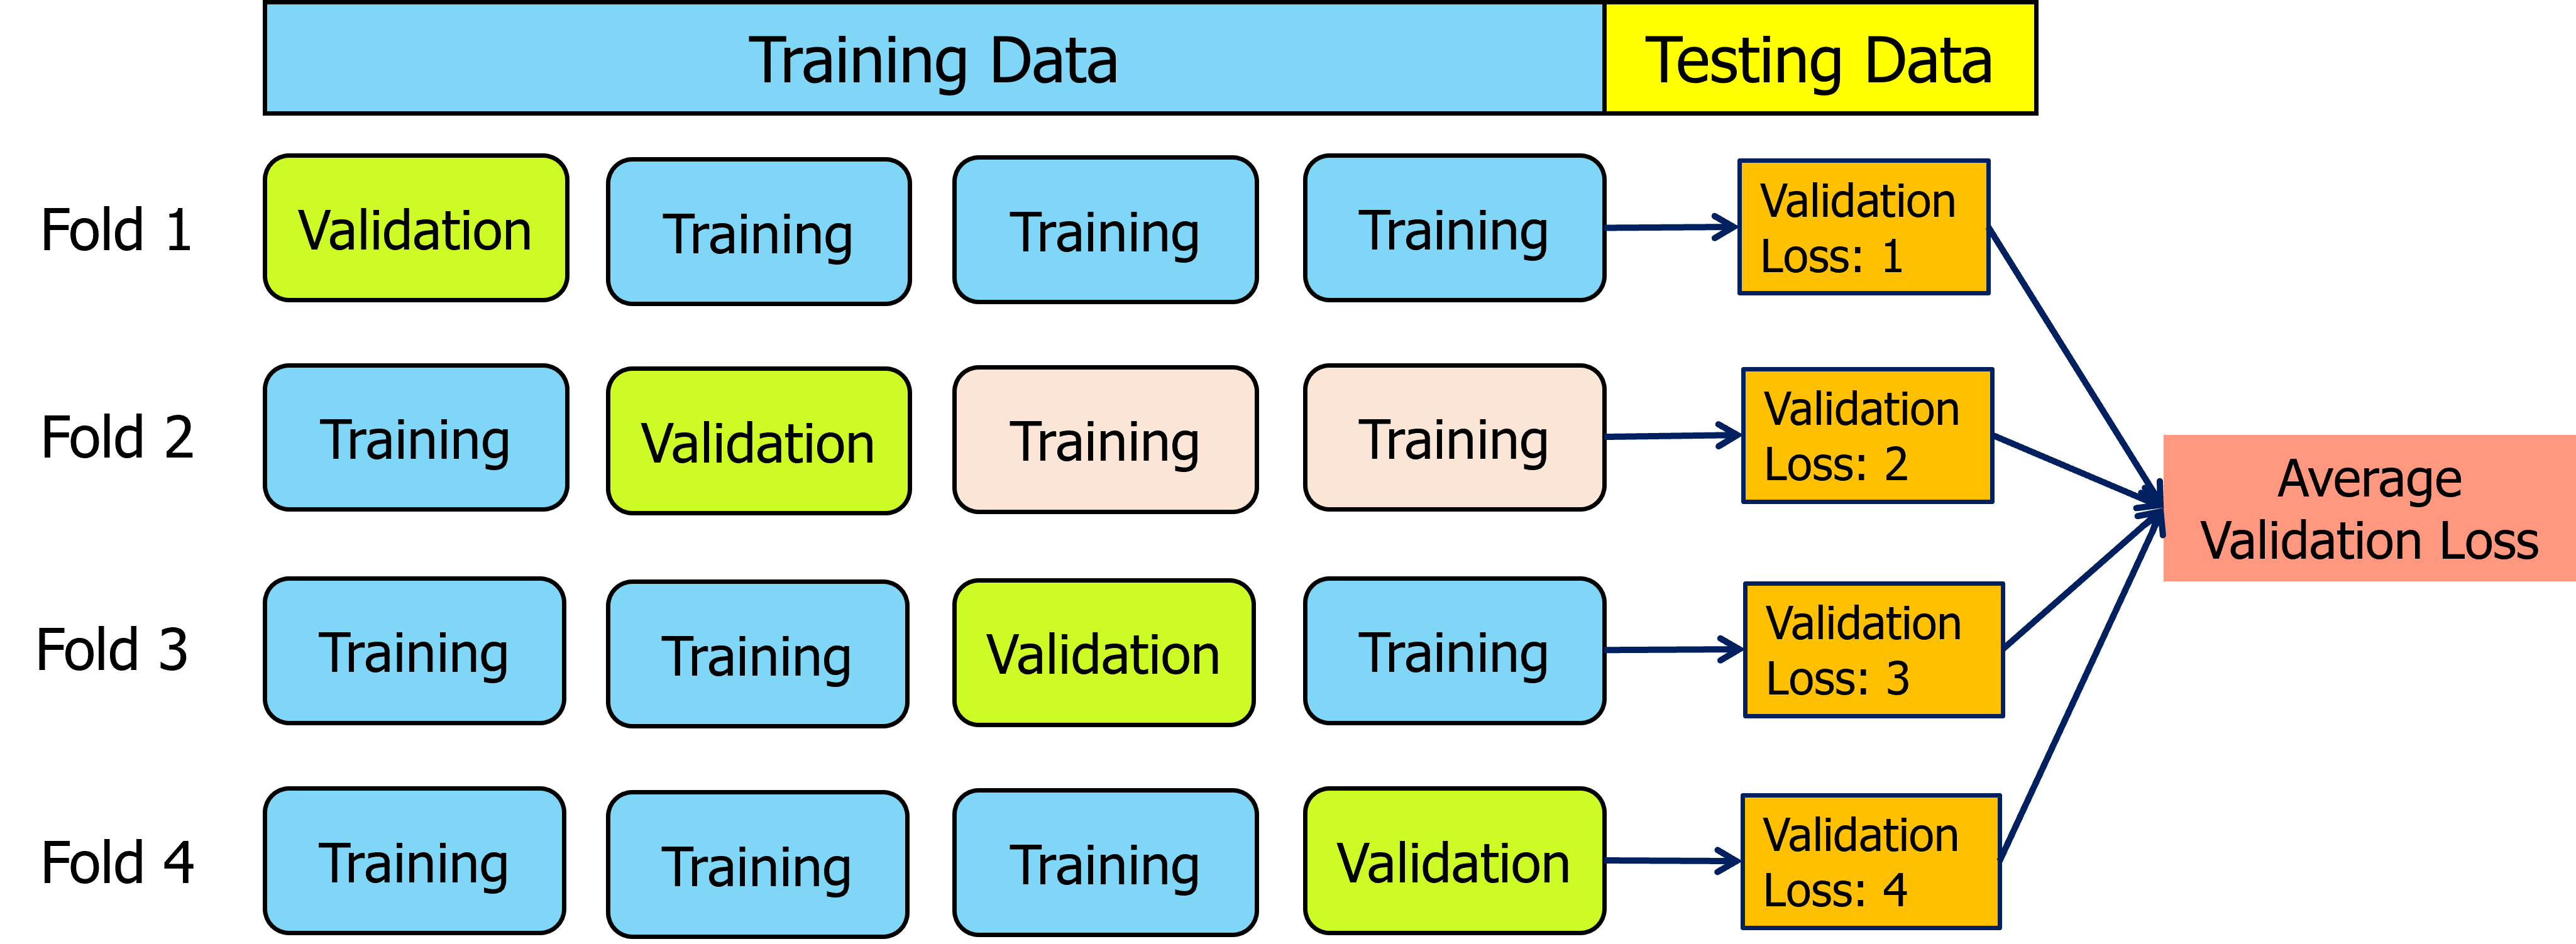
\includegraphics[width=\linewidth]{images/k-foldcrossval.png}
    \caption{K-fold Cross-Validation: The training data is divided into multiple subsets (folds). Each fold takes a turn as the validation set while the rest are used for training. The final validation score is the average of validation losses across all folds.}
    \label{fig:kfold}
\end{figure}


\begin{lstlisting}[language=Python]
# Example Python code for k-fold cross-validation with shuffling
from sklearn.model_selection import KFold
import numpy as np

data = np.array([...])  # Example data array
kfold = KFold(n_splits=5, shuffle=True, random_state=42)

for train, test in kfold.split(data):
    # Apply training and testing here
\end{lstlisting}
% --------------------------------- Data Processing and Feature Engineering ----------------------

\section{Data Processing and Feature Engineering}
\begin{itemize}
    \item \textbf{Normalization and Vectorization:} Techniques to scale and convert data into a format suitable for deep learning.
    \item \textbf{Handling Missing Values:} Strategies for dealing with incomplete datasets.
    \item \textbf{Feature Engineering:} Discuss how effective features can be engineered from data to improve model performance.
\end{itemize}
\section*{Perfromance Metrics}
 % Ensure longtable package is included in the preamble
\begin{longtable}{|p{0.2\textwidth}|p{0.3\textwidth}|p{0.45\textwidth}|}
\hline
\textbf{Metric} & \textbf{Equation} & \textbf{Python Code} \\
\hline
Mean Squared Error (MSE): Measures the average squared difference between observed and predicted values. &
\( \text{MSE} = \frac{1}{n} \sum_{i=1}^{n} (y_i - \hat{y}_i)^2 \) &
\begin{lstlisting}[language=Python, numbers=none]
import numpy as np

def calculate_mse(y_true, y_pred):
    return np.mean((y_true - y_pred) ** 2)

# Example
y_true = np.array([1, 2, 3, 4, 5])
y_pred = np.array([1.1, 2.1, 2.9, 3.8, 5.2])
mse = calculate_mse(y_true, y_pred)
print("MSE:", mse)
\end{lstlisting} \\
\hline
Root Mean Squared Error (RMSE): The square root of MSE, providing error in the same unit as the target. &
\( \text{RMSE} = \sqrt{\text{MSE}} \) &
\begin{lstlisting}[language=Python, numbers=none]
def calculate_rmse(y_true, y_pred):
    return np.sqrt(np.mean((y_true - y_pred) ** 2))

rmse = calculate_rmse(y_true, y_pred)
print("RMSE:", rmse)
\end{lstlisting} \\
\hline
Nash-Sutcliffe Efficiency (NSE): Compares model performance to the mean of observed data. Higher values (close to 1) are better. &
\( \text{NSE} = 1 - \frac{\sum_{i=1}^{n} (y_i - \hat{y}_i)^2}{\sum_{i=1}^{n} (y_i - \bar{y})^2} \) &
\begin{lstlisting}[language=Python, numbers=none]
def calculate_nse(y_true, y_pred):
    numerator = np.sum((y_true - y_pred) ** 2)
    denominator = np.sum((y_true - np.mean(y_true)) ** 2)
    return 1 - (numerator / denominator)

nse = calculate_nse(y_true, y_pred)
print("NSE:", nse)
\end{lstlisting} \\
\hline
Coefficient of Determination (R$^2$): Represents the proportion of the variance in the observed data explained by the model. &
\( R^2 = 1 - \frac{\sum (y_i - \hat{y}_i)^2}{\sum (y_i - \bar{y})^2} \) &
\begin{lstlisting}[language=Python, numbers=none]
def calculate_r2(y_true, y_pred):
    ss_res = np.sum((y_true - y_pred) ** 2)
    ss_tot = np.sum((y_true - np.mean(y_true)) ** 2)
    return 1 - (ss_res / ss_tot)

r2 = calculate_r2(y_true, y_pred)
print("R2:", r2)
\end{lstlisting} \\
\hline
Percent Bias (\%Bias): Measures the average tendency of simulated data to be larger or smaller than observed values. &
\( \%\text{Bias} = \frac{\sum (y_i - \hat{y}_i)}{\sum y_i} \times 100 \) &
\begin{lstlisting}[language=Python, numbers=none]
def calculate_percent_bias(y_true, y_pred):
    return 100 * np.sum(y_true - y_pred) / np.sum(y_true)

percent_bias = calculate_percent_bias(y_true, y_pred)
print("%Bias:", percent_bias)
\end{lstlisting} \\
\hline
Accuracy (for Classification): Percentage of correctly classified instances. &
\( \text{Accuracy} = \frac{\text{Correct Predictions}}{\text{Total Predictions}} \) &
\begin{lstlisting}[language=Python, numbers=none]
def calculate_accuracy(y_true, y_pred):
    return np.sum(y_true == y_pred) / len(y_true)

# Example for classification
y_true_class = np.array([0, 1, 1, 0, 1])
y_pred_class = np.array([0, 1, 0, 0, 1])
accuracy = calculate_accuracy(y_true_class, y_pred_class)
print("Accuracy:", accuracy)
\end{lstlisting} \\
\hline
\end{longtable}
% --------------------------------- Universal Workflow of Deep Learning ---------------

\section{Universal Workflow of Deep Learning}
\label{sc: udl}
Outline the standard steps involved in a deep learning project:
\begin{enumerate}
    \item Defining the problem and the data inputs.
    \item Choosing metrics and methods for evaluation.
    \item Engineering features from the data.
    \item Developing models to combat overfitting.
    \item Implementing interpretive mechanisms to understand model predictions.
\end{enumerate}



% ------------------------------------ SUMMARY ----------------------------------------------
\section{Summary}
Summarize the key points discussed in the chapter and reiterate the importance of a systematic approach to developing deep learning models.



% \section{Keras APIs to build DL models}
Follow this link: https://machinelearningmastery.com/keras-functional-api-deep-learning/
https://www.activestate.com/resources/quick-reads/what-is-a-keras-model/

An API (Application Programming Interface) is a set of tools and functions that allow you to interact with a software or framework. In simple terms, think of an API as a menu at a restaurant: it tells you what dishes (functions) you can order (use), without needing to know how they are prepared (the underlying implementation). In the context of Keras, APIs let you define, build, and train deep learning models easily, without knowing much about how the Keras functions are built.

Types of Keras APIs for Building Deep Learning Models
Keras offers two main APIs for building models:

Sequential API: A simple, linear stack of layers where each layer has one input and one output.
Functional API: A more flexible approach where you can define complex architectures like multi-input, multi-output models, or models with shared layers.
\subsection{Sequential API}
The Sequential API is the easiest and most intuitive way to build a model. You stack layers one after another, like building blocks. It works well when your model has a straightforward flow of data from input to output without branching.

Why is it popular?
Simplicity: Perfect for beginners or for straightforward tasks.
Fast to implement: Requires minimal coding effort.
Readable: Easy to understand and debug.
Example in Rainfall-Runoff Modeling
Suppose you want to predict river runoff based on rainfall data. Using the Sequential API, you can create a simple feedforward neural network where data flows through layers in one direction:



\subsection{Functional API}
The Functional API is more flexible and allows you to define complex architectures. Unlike the Sequential API, you can connect layers in arbitrary ways, such as branching or merging data flows.

Why do hydrologists need it?
Complex Models: You may need models with multiple inputs (e.g., rainfall from different regions and soil moisture data) or multiple outputs (e.g., runoff and evaporation).
Shared Layers: Useful when you want the same computation applied to different inputs, such as rainfall data from multiple time steps.
Custom Architectures: Models with residual connections (like in ResNet) or attention mechanisms often require the Functional API.
Example in Rainfall-Runoff Modeling
Let’s say you want to predict runoff using rainfall data from two separate regions (Region A and Region B). Each region’s data requires a different processing branch before being combined for the final prediction:

Here, rainfall data from Region A and Region B are processed separately but combined to predict runoff. This architecture is only possible with the Functional API. 
\input{chapters/keras and tf/tf}
\section{Classifying Drought Severity: a Binary Classification Example}
% \chapter{Autoencoders}
\label{chap:acn}


% \include{chapters/machine_learning}
% \include{chapters/deep_learning_applications}
% \include{chapters/case_studies}

% Appendices and index would go here
\appendix
% \include{chapters/appendix}

\end{document}
